\documentclass[a4paper,11pt,twoside,titlepage]{ThesisStyle}

\include{formatAndDefs}
\usepackage[english,francais]{babel}
\usepackage[utf8]{inputenc} % comment out for lualatex/xelatex
\usepackage[T1]{fontenc}    % comment out for lualatex/xelatex
\usepackage{titlesec}
\usepackage{hyperref}
\usepackage{graphicx}
\usepackage{listings}
\renewcommand{\lstlistingname}{Code source}
\usepackage{color}
\definecolor{lightgray}{rgb}{.9,.9,.9}
\definecolor{darkgray}{rgb}{.4,.4,.4}
\definecolor{purple}{rgb}{0.65, 0.12, 0.82}
\definecolor{ocher}{rgb}{1, 0.5, 0} % #FF7F00 -> rgb(239, 169, 0)
\definecolor{green}{rgb}{0, 0.5, 0} % #007C00 -> rgb(0, 124, 0)
\definecolor{olive}{rgb}{0.17,0.59,0.20}
\definecolor{brown}{rgb}{0.69,0.31,0.31}

\lstdefinelanguage{CSS}{
  keywords={color,background-image:,margin,padding,font,weight,display,position,top,left,right,bottom,list,style,border,size,white,space,min,width, transition:, transform:, transition-property, transition-duration, transition-timing-function},	
  sensitive=true,
  morecomment=[l]{//},
  morecomment=[s]{/*}{*/},
  morestring=[b]',
  morestring=[b]",
  alsoletter={:},
  alsodigit={-}
}
\lstdefinelanguage{JavaScript}{
  morekeywords={typeof, new, true, false, catch, function, return, null, catch, switch, var, if, in, while, do, else, case, break},
  morecomment=[s]{/*}{*/},
  morecomment=[l]//,
  morestring=[b]",
  morestring=[b]'
}
\lstdefinelanguage{HTML5}{
  language=html,
  sensitive=true,	
  alsoletter={<>=-},	
  morecomment=[s]{<!-}{-->},
  tag=[s],
  otherkeywords={
  % General
  >,
  % Standard tags
	<!DOCTYPE,
  </html, <html, <head, <title, </title, <style, </style, <link, </head, <meta, />,
	% body
	</body, <body,
	% Divs
	</div, <div, </div>, 
	% Paragraphs
	</p, <p, </p>,
	% scripts
	</script, <script,
  % More tags...
  <canvas, /canvas>, <svg, <rect, <animateTransform, </rect>, </svg>, <video, <source, <iframe, </iframe>, </video>, <image, </image>, <header, </header, <article, </article
  },
  ndkeywords={
  % General
  =,
  % HTML attributes
  charset=, src=, id=, width=, height=, style=, type=, rel=, href=,
  % SVG attributes
  fill=, attributeName=, begin=, dur=, from=, to=, poster=, controls=, x=, y=, repeatCount=, xlink:href=,
  % properties
  margin:, padding:, background-image:, border:, top:, left:, position:, width:, height:, margin-top:, margin-bottom:, font-size:, line-height:,
	% CSS3 properties
  transform:, -moz-transform:, -webkit-transform:,
  animation:, -webkit-animation:,
  transition:,  transition-duration:, transition-property:, transition-timing-function:,
  }
}
\lstdefinelanguage{haml}{
  morestring=[b]',
  morestring=[b]",
  sensitive=true,
  keywordsprefix=\%,
  alsoletter=\%
}
\lstdefinelanguage{Gherkin}{
  ndkeywords={Feature:, Scenario:},
  keywords={Given, And, When, Then},
  alsoletter=\:,
  comment=[l]@
}
\lstdefinelanguage{Rails}{
  language=Ruby,
  sensitive=true,	
  morestring=[d]/,
  ndkeywords={
    %controller
    params, before_action, before_filter, render, redirect_to,
    %model
    scope, where, validates, delegate, belongs_to, has_one, has_many, includes, order},
  morekeywords={private, public, protected, include}
}
\lstset{
  %backgroundcolor=\color{lightgray},
  extendedchars=true,
  basicstyle=\footnotesize\ttfamily,
  showstringspaces=false,
  showspaces=false,
  numbers=left,
  numberstyle=\tiny,
  numbersep=9pt,
  tabsize=2,
  breaklines=true,
  showtabs=false,
  captionpos=b,
  frame=single,
  frameround=fttt,
  keywordstyle=\color{blue}\bfseries,
  ndkeywordstyle=\color{green}\bfseries,
  identifierstyle=\color{black},
  commentstyle=\color{purple}\ttfamily,
  stringstyle=\color{brown}\ttfamily,
  inputencoding=utf8,
  extendedchars=true,
  literate=
  {á}{{\'a}}1 {é}{{\'e}}1 {í}{{\'i}}1 {ó}{{\'o}}1 {ú}{{\'u}}1
  {Á}{{\'A}}1 {É}{{\'E}}1 {Í}{{\'I}}1 {Ó}{{\'O}}1 {Ú}{{\'U}}1
  {à}{{\`a}}1 {è}{{\`e}}1 {ì}{{\`i}}1 {ò}{{\`o}}1 {ù}{{\`u}}1
  {À}{{\`A}}1 {È}{{\'E}}1 {Ì}{{\`I}}1 {Ò}{{\`O}}1 {Ù}{{\`U}}1
  {ä}{{\"a}}1 {ë}{{\"e}}1 {ï}{{\"i}}1 {ö}{{\"o}}1 {ü}{{\"u}}1
  {Ä}{{\"A}}1 {Ë}{{\"E}}1 {Ï}{{\"I}}1 {Ö}{{\"O}}1 {Ü}{{\"U}}1
  {â}{{\^a}}1 {ê}{{\^e}}1 {î}{{\^i}}1 {ô}{{\^o}}1 {û}{{\^u}}1
  {Â}{{\^A}}1 {Ê}{{\^E}}1 {Î}{{\^I}}1 {Ô}{{\^O}}1 {Û}{{\^U}}1
  {œ}{{\oe}}1 {Œ}{{\OE}}1 {æ}{{\ae}}1 {Æ}{{\AE}}1 {ß}{{\ss}}1
  {ç}{{\c c}}1 {Ç}{{\c C}}1 {ø}{{\o}}1 {å}{{\r a}}1 {Å}{{\r A}}1
  {€}{{\EUR}}1 {£}{{\pounds}}1
}


% \usepackage[nomain,acronym,xindy,toc]{glossaries}
% \makeglossary
% \usepackage[xindy]{imakeidx}
% \makeindex

\newcommand{\fwshort}{RSnap}
\newcommand{\fwlong}{Plateforme web pour accompagner l'apprentissage de la programmation par les 10 - 14 ans}
\newcommand{\HRule}{\rule{\linewidth}{0.5mm}}
\newcommand{\hRule}{\rule{\linewidth}{0.1mm}}
\def \doctitle {Plateforme web pour accompagner l'apprentissage de la programmation par les 10 - 14 ans}
\def \docsubtitle {}
\def \doccourssigle{LINGI2990}
\def \doccourstitle{Mémoire}
\def \docauthor {Gaetan \textsc{Collart}\\\emph{Année :} INFO 22 MS\\\emph{Noma :} 66-20-07-00 \and Simon \textsc{Claessens}\\\emph{Année :} INFO 22 MS\\\emph{Noma :} 31-06-07-00}
\def \docprofessor{Chantal \textsc{Poncin} \and Pierre \textsc{Schaus}}
%\def \docassistant{Nicolas \textsc{Cardozo Alvarez}}

\author{Gaetan Collart \and Simon Claessens}
\title{Plateforme web pour accompagner l'apprentissage de la programmation par les 10 - 14 ans}

\usepackage{mdwlist} %reduce itemize item spacing
\usepackage{placeins} %De­fines a \FloatBar­rier com­mand, be­yond which floats may not pass

\usepackage[plain]{fancyref}
\def\fref{\Fref} % treat all \frefs as \Frefs
% Define 'lst' delimiter for fancyref
\newcommand*{\fancyreflstlabelprefix}{lst}
\newcommand*{\Freflstname}{\lstlistingname}
\newcommand*{\freflstname}{\MakeLowercase{\lstlistingname}}
\Frefformat{vario}{\fancyreflstlabelprefix}%
 {\Freflstname\fancyrefdefaultspacing#1#3}

\frefformat{vario}{\fancyreflstlabelprefix}%
 {\freflstname\fancyrefdefaultspacing#1#3}
\Frefformat{plain}{\fancyreflstlabelprefix}%
 {\Freflstname\fancyrefdefaultspacing#1}
\frefformat{plain}{\fancyreflstlabelprefix}%%
 {\freflstname\fancyrefdefaultspacing#1}

%\includeonly{content/4-prerequis/background, content/5-related_work/travail}
%======================
%	DOCUMENT
%======================
%include{content/12-glossary/glossary}
\begin{document}
%\dominitoc


\maketitle
%\input{titlepage}

\pagenumbering{arabic}

\section*{Résumé}
Ordinateurs, smartphones, tablettes, montres connectées, voitures intelligentes, de nos jours, les technologies informatiques sont partout. Les exemples dans la vie quotidienne sont innombrable. En revanche le nombre de personne qui comprennent leurs fonctionnements lui le devient de plus en plus. \\

La programmation prend de plus en plus de place dans notre vie. hors, quelle place est laissée pour son apprentissage dans les programmes officielle ? De plus, l'apprentissage de la programmation pourrait être bénéfique pour les jeunes. En effet la pratique de la programmation forge une logique et un esprit analytique.\\

% programmation
L'idée poursuivie dans ce mémoire est de fournir une plateforme d'apprentissage de la programmation orienté vers les école. Ce travail présente une plateforme d'apprentissage de la programmation articulée autour de missions ludique et de défits de créatifs.\\

La plateforme est basé sur des technologies web pour être le plus portable possible. Elle intègre un environnement de programmation par blocs pour permettre à tous de rentrer rapidement dans les activités. De plus cette plateforme est entièrement en français ce qui n'existait pas encore actuellement.\\

Des enfants lors d'expériences ont eu l'occasion de tester cette plateforme ce qui a permis de tester de manière pratique cette application. Elle a rencontré un franc succès ce qui laisse à penser que cette solution fonctionne.


\begin{otherlanguage}{english}
\section*{Abstract}
Computers, smart-phones, tablets, connected watches, smart cars, nowadays, computer technologies are everywhere. Examples in everyday life are countless. However the number of people who understand what they use become more and more countable. \\

Programming is becoming more important in our lives. But, what place is reserved for this learning in the official programs? In addition, learning programming could be beneficial for young people. Indeed, the practice of programming train a logical and analytical mind. \\

% programming
The idea pursued in this paper is provide a school oriented programming platform. This work presents a platform for learning programming build around fun missions and creative challenge. \\

The platform is based on web technologies to be as portable as possible. It includes a blocks based programming environment, it allows everyone to begin quickly activities. In addition, this platform is entirely in French which currently does not exist. \\

Children had an opportunity to test this platform during an experiment. It allows to test this application in a practical way. It was a success which suggests that this solution works.
\end{otherlanguage}

\section*{Remerciements}
Dans cette partie les auteurs tiennent à remercier tout particulièrement certaines personnes et organisations.\\

Le projet \gls{snap} et toutes les personnes qui lui donnent vie. Sans ce projet ou sans son caractère open source ce mémoire n'aurait pas été aussi abouti.\\

Poncin Chantal et Schaus Pierre pour nous avoir guidé et soutenu tout au long de ce mémoire.\\

Tous les lecteurs: Claessens Yves, Collart Eric, Deltour Christine, Poncelet Thibault, Questiaux Isabelle; pour avoir relu et permis de réduire le nombre de fautes d'orthographe, d'améliorer le style rédactionnel et la qualité technique.

L'initiative KidsCode pour nous avoir accueilli, permis de mener une expérience chez eux et pour leur compte rendu de cette expérience qui nous a bien orientés.

L'initiative Science Infuse qui nous a permis de mener des expériences avec 4 classes d'enfants ce qui fut très bénéfique à la qualité de la solution qui est proposée.

%\faketableofcontents
\tableofcontents
%\listoffigures


%\mainmatter
\chapter{Introduction}
\section{Contexte}
\label{intro-context}
Dans un monde où la pédagogie est un sujet de société et où l'informatique est omniprésente, on s'étonne de n'observer que peu d'interactions entre ces deux sujets. Il existe toutefois quelques recherches et initiatives. Il faut encore distinguer celles qui concernent l'informatique dans son ensemble et celles qui se portent sur la programmation.\\

Il existe deux écoles d'apprentissage de la programmation. La première prône l'apprentissage de la programmation directement avec des langages de programmation classique. D'autres préfèrent des langages simplifiés ; par exemple la programmation par \glspl{bloc}.

Ces deux écoles se différencient essentiellement par rapport au public qu'elles visent. Une programmation par \glspl{bloc} sera plus simple dans un premier temps et donc sera mieux adaptée aux enfants plus jeunes n'ayant aucune expérience avec la programmation. Une approche avec un langage complet comme Python sera plus adaptée pour des enfants plus âgés ou ayant déjà une expérience.\\

Des initiatives sont disponibles dans d'autres pays et d'autres langues. Mais aucune de ces initiatives n'a été conçue pour un public francophone.



%Dans le domaine de la recherche, nous retiendrons essentiellement une publication de la communauté européenne qui stipule que l'apprentissage de la programmation apporte un soutien a la structuration de raisonnement logique.\\ %TODO revoir la formulation pourquoi que l'Europe?

%Nous clôturerons cette partie avec un constat, dans une société où l'informatique occupe une place prédominante, nous constatons que la connaissance de la programmation n'est pas encore beaucoup valorisée et stimulée.  %TODO ??

\section{Problème}
\label{into-problem}
Le but de ce travail est de promouvoir l'apprentissage de la programmation auprès des plus jeunes. En effet là nous avons vu dans la section \ref{intro-context} qu'il y a un manque de moyens pédagogiques dans ce domaine. Ce travail propose une adaptation d'un programme informatique existant Snap! mais en amenant cela dans une interface web et soutenu par un serveur. Ce travail vise donc à produire une nouvelle plateforme spécialisée dans l'apprentissage de la programmation accessible à tous, aussi bien les professeurs que les élèves. L'enseignant pourra grâce à l'application donner des cours de programmation à ses classes sans avoir de connaissances particulières.

En plus de l'application, un ensemble de missions simple a été réalisé et testé sur des enfants pour montrer que ce projet est viable. Les missions proposées devaient avoir aussi bien des objectifs pédagogiques que ludiques.

\section{Motivation}
\label{intro-motivation}
L'éducation des jeunes à la programmation peut être bénéfique à la société sur de nombreux points comme : la structuration logique de l'esprit, une meilleure compréhension de l'environnement ou encore un meilleur départ des enfants s'ils souhaitent se lancer dans l'informatique.

L'Europe nous indique que la programmation est un très bon exercice pour la structuration logique de l'esprit. En effet, la programmation demande beaucoup de rigueur, une erreur, un oubli dans la structuration ou dans la syntaxe entraine directement une erreur. L'algorithme vu comme un enchaînement de commande ou d'instruction est un exercice de raisonnement logique.

Dans les cours de technologie, par exemple, plusieurs professeurs essayent d'apprendre l'informatique aux jeunes. Mais par manque de supports, d'applications adéquates et probablement aussi par manque de connaissances dans ce domaine, ils n'enseignent que trop peu la programmation et se contentent de la bureautique. Ce travail peut fournir une aide précieuse pour tous ces professeurs en mettant à leur disposition une plateforme qui les soutiendrai dans leur enseignement.

La technologie et l'informatique sont partout, pourtant bon nombre de personnes ne comprennent pas comment tout ça fonctionne. Il serait donc intéressant que les enfants ai une idée de comment fonctionnent les objets de leur quotidien.

\section{Objectifs}
\label{intro-objectifs}
Le but de ce travail est de fournir une interface pour apprendre aux jeunes la programmation. Cette interface devra être dans un navigateur pour des questions de facilité d'utilisation. En effet, cette application est orientée vers les écoles et donc il faut une utilisation simple et intuitive faite pour des personnes n'ayant pas ou peu de connaissances en programmation et le minimum en informatique en général. L'intérêt d'une plateforme web est aussi de ne devoir rien installer sur les ordinateurs.

Il faut également deux types d'interface, une pour les jeunes où toutes les fonctions inutiles sont retirées ainsi que les options pour modifier l'interface. Une pour les professeurs pour leur permettre d'avoir accès aux fonctions qui permettent de cacher des blocs et des scripts.

Un serveur qui va permettre aux jeunes de réaliser les missions et de les soumettre. Aux professeurs, ce site va permettre en plus de centraliser les travaux des jeunes, mais également de permettre d'ordonnancer les missions et de mettre des verrous sur les missions.

Nous souhaitons apporter une plate-forme facile à utiliser pour un professeur qui ne programme pas et pour des enfants pour apprendre la programmation. 

Nous souhaitons avoir une interface dans un navigateur qui est en lien avec un serveur sur lequel sont stockées les données.

\section{Approche}
\label{intro-approche}
%TODO \gls{Rsnap}
L'application développée dans le cadre de ce travail est nommée \gls{rsnap}.

\paragraph{La plateforme} La plateforme sera implémentée par une combinaison entre un environnement de programmation existant \gls{snap} \cite{snap} et un site web en \gls{rails} \cite{rails}. Cette combinaison permet d'avoir une plateforme accessible par tous les ordinateurs ayant accès à internet et un navigateur récent.

La plateforme devant aussi permettre la création de contenu par les professeurs, il sera nécessaire d'introduire des \glspl{role} différent pour ceux-ci et les jeunes.

\paragraph{Le contenu} Le contenu initial fourni sera une série de \glspl{mission} qui se succède, la fin de l'une débloquant la suivante. Cette série d'exercices introduira les concepts nécessaires à la création d'un jeu plus conséquent. Ce jeu sera un jeu de poursuite permettant aux jeunes de jouer entre eux.

\section{Contributions}
\label{intro-contribution}
Cette section présente les différentes contribution de ce travail à l'existant. Nous retiendront principalement: un outils francophone pour apprendre la programmation, une plateforme intégrée orienté pour l'enseignement et la combinaison d'outils existant.

\paragraph{Un outil francophone} Comme introduit dans la section \ref{into-problem} il n'existait pas encore ou peu de matériel francophone pour soutenir l'apprentissage de la programmation. Rsnap est une plateforme entièrement francophone et les traductions de Snap! on été finie et améliorée dans le cadre de ce travail.

\paragraph{Une plateforme utilisable} Aucune plateforme n'est actuellement disponible pour l'apprentissage de la programmation. Rsnap se veut être orienté pour l'apprentissage dans l'enseignement traditionnel. Ceci en intégrant une gestion de classe, une progression contrôlable par l'enseignant. Rsnap à été pensée dès le début pour que les élèves puissent l'utilisé de la manière la plus autonome possible.

\paragraph{Combinaison d'outils existant} Dans le cadre de ce mémoire les ressources tant au niveau temps que matérielle sont comptée. Ce travail montre également que à l'aide de plateforme libre existante et de technologie tel que JavaScript ou encore Ruby on Rails, il est possible de crée une plateforme d'apprentissage aboutie.




%
%
%
%
%%TODO Programmation francophone, plateforme, montrer que c'est facile qu'il y a deja plein d'outils, 
%Papier sur les biens faits de l'apprentissage de la programmation sur l'esprit logique.
%
%Le projet SNAP est à l'origine maintenu par jmoening. C'est la principale contribution au projet. Dans ce travail, certaines parties ont pu être intégrées au projet, par exemple la traduction des aides en français a pu être ajoutée au projet de jmoening. Deux autres pull request sont en court. La première concerne l'ajout de rôle pour pouvoir modifier l'interface facilement en fonction des rôles que l'on souhaite avoir. La seconde porte sur une traduction automatisée de l'interface. Une autre pourrait encore être proposée pour les fonctions d'importation et d'exportation qui ont été ajoutées pour ce travail.
%
%Jimoegning bref lui :)
%
%Tous les autres intervenants
%
%Écoles ?
%
%Printemps des sciences ?

\section{Plan du mémoire}
La suite de ce mémoire se divise de la manière suivante:

\paragraph{Connaissances nécessaires}
Ce chapitre introduit le bagage technique nécessaire à la bonne compréhension de ce travail. Il commence par quelques prérequis, puis introduit \gls{snap} et enfin parle plus en détail de \gls{rails}.

\paragraph{Travaux associés}
Ce chapitre parle de l'état de l'art dans le monde. Il présente l'avancée de l'apprentissage de la programmation dans le monde. Ensuite, il présente quelques grandes initiatives similaires à celle de ce travail. Après quoi, il introduit les différents langages de programmation enseignés aux jeunes. Et se finit par une liste de concepts différenciateurs qui permet de définir une initiative de manière unique.

\paragraph{Définition de la problématique}
Ce chapitre présente la position de ce mémoire par rapport au chapitre précédent. Il positionne \gls{rsnap} par rapport aux concepts différenciateurs introduits dans les travaux associés. Et pour finir, il décrit les choix technologiques faits dans le cadre de ce travail.

\paragraph{Solution}
Ce chapitre décrit la plateforme \gls{rsnap} implémentée dans le cadre de ce mémoire.
Il commence par décrire les \glspl{mission} qui ont été crées pour ce travail. Il parle ensuite des modifications apportées à \gls{snap} pour les besoins du mémoire. Il fini par décrire la partie web de \gls{rsnap}.

\paragraph{Validation}
Ce chapitre présente la validation de l'application. Il commence par les tests sur l'application \gls{rsnap}. Il présente ensuite les expériences qui ont été menées. Et fini par l'analyse des formulaires proposée aux participants de l'expérience.

\paragraph{Conclusion}
Ce chapitre conclut ce travail, compare les objectifs attendus et atteints, les points plus faibles et les points forts de ce mémoire. %TODO à retravailler quand elle sera écrite

\paragraph{Futures amélioration}
Ce chapitre décrit ce qui serait utile de faire dans la continuité de ce travail. Ce sont des améliorations qui n'ont pas pu être réalisées soit par manque de temps soit parce qu'elles sont apparues dans l'analyse des expériences.



%==========================
%       PART 1
%==========================
\chapter{Connaissances nécessaires}
Ce chapitre commencera par présenter de manière succincte les prérequis pour pouvoir suivre ce document. Ensuite, une description plus technique présentera les outils utilisés.

\section{Prérequis}
Les connaissances nécessaires à la bonne compréhension de ce travail vont être développées dans cette partie.

\paragraph{Snap!}
Commençons par la partie portant sur Snap! BYOB. 

Cette application est implémentée en JavaScript. Donc, de bonnes connaissances dans ce langage de programmation seront un atout pour comprendre les logicielles utilisés et les apports et modifications apportées à ceux-ci.

Cette application utilise une programmation dite par bloc. Le principe est d'empiler des blocs qui représente des opérations. Une fois ces blocs assemblés, il représente un programme exécutable. Un exemple de programme est disponible sur la figure \ref{fig:prog}

\begin{figure}[]
  \begin{center}
  
\includegraphics[width=\textwidth]{content/4-prerequis/images/snap}
        \caption{Exemple de programmation par bloc}
    \label{fig:prog}
  \end{center}
\end{figure}


\paragraph{Ruby on Rails}
La plateforme web est implémentée en Ruby on Rails qui est le framework le plus utilisé pour la création de site web en Ruby. 

Des connaissance sur l'architecture de type modèle-vue-contrôleur sont nécessaire. 

L'utilisation de gems, bibliothèque logicielle, demande des base en développement Ruby. Plus de détails techniques seront donnés dans la suite de ce chapitre \ref{techno}. %TODO ajouter gem au glossaire

\paragraph{Pédagogie}
Pour l'apprentissage de la programmation aux jeunes, des notions de pédagogie sont également nécessaires. 
Les programmes d'apprentissages existants permettent de définir les concepts considérés comme acquis par les élèves. La communication avec les jeunes demande un vocabulaire adapté. Tout ceci s'avère important pour les choix de design d'interface. Par exemple, suivant leur âge, les jeunes ne seront pas stimulés par les mêmes images ou couleurs.

\section{Snap!}
Cette partie donne un aperçu de l'application qui est utilisée dans ce travail. La présentation de \gls{snap} \cite{snap} se divise en plusieurs sections. La première explique les différents types de \glspl{bloc} et comment ils sont implémentés. L'étape suivante explique l'exécution d'un programme. Ensuite vient l'affichage des différents éléments de \gls{snap}.

\subsection{Utilisation}
%Cette partie présente comment utiliser \gls{snap} pour faire un programme. Elle présentera le différente division de l'interface graphique ainsi que leur utilité. Pour ce faire les images \ref{fig:snap interface} et \ref{fig:prog} sont utilisé, la première présente les différentes divisions de l'interface, la seconde montre un exemple concret de programme.
Cette partie va illustrer comment réaliser un programme avec \gls{snap}. Ceci permet de découvrir les différentes zones de l'interface de \gls{snap} et leurs utilisations. Cette explication se base sur les images \ref{fig:snap interface} et \ref{fig:prog}.

\paragraph{Personnages}
Pour réaliser un programme avec \gls{snap}, il faut commencer par savoir combien de personnages sont souhaités. Les personnages s'appellent des \textit{\glspl{sprite}} et sont visibles dans la \textit{zone des \glspl{sprite}} de la figure \ref{fig:snap interface}. On peut voir dans le programme de l'image \ref{fig:prog}, que deux personnages sont présents : un chien et un chat. Le bouton blanc au dessus de la \textit{zone de \glspl{sprite}} permet d'ajouter des personnages.

\paragraph{Scripts}
Après avoir ajouté le nombre de personnages souhaité, il faut maintenant faire des \glspl{script} qui seront le code du programme. Les \glspl{script} sont assemblés, par glissé-déposé, dans la \textit{zone d'édition} au centre de l'interface. Ceux-ci sont construits à l'aide de \glspl{bloc} qui se trouvent dans la \textit{zone des \glspl{bloc} sources}. Cette zone contient tous les \glspl{bloc} disponibles classés par catégorie suivant l'action du \gls{bloc}.

\paragraph{Monde}
Une fois le programme fini, le drapeau vert dans la \textit{barre d'outils}, lance le programme. Quand le programme est lancé, les actions des \glspl{script} sont visibles dans la \textit{scène}. Cette zone représente le monde dans lequel vont évoluer les personnages. On peut y mettre un fond comme arrière-plan ou simplement le laisser blanc comme dans l'exemple, ceci se fait via le bouton stage de la \textit{zone de \glspl{sprite}}.

\begin{figure}
  \begin{center}
  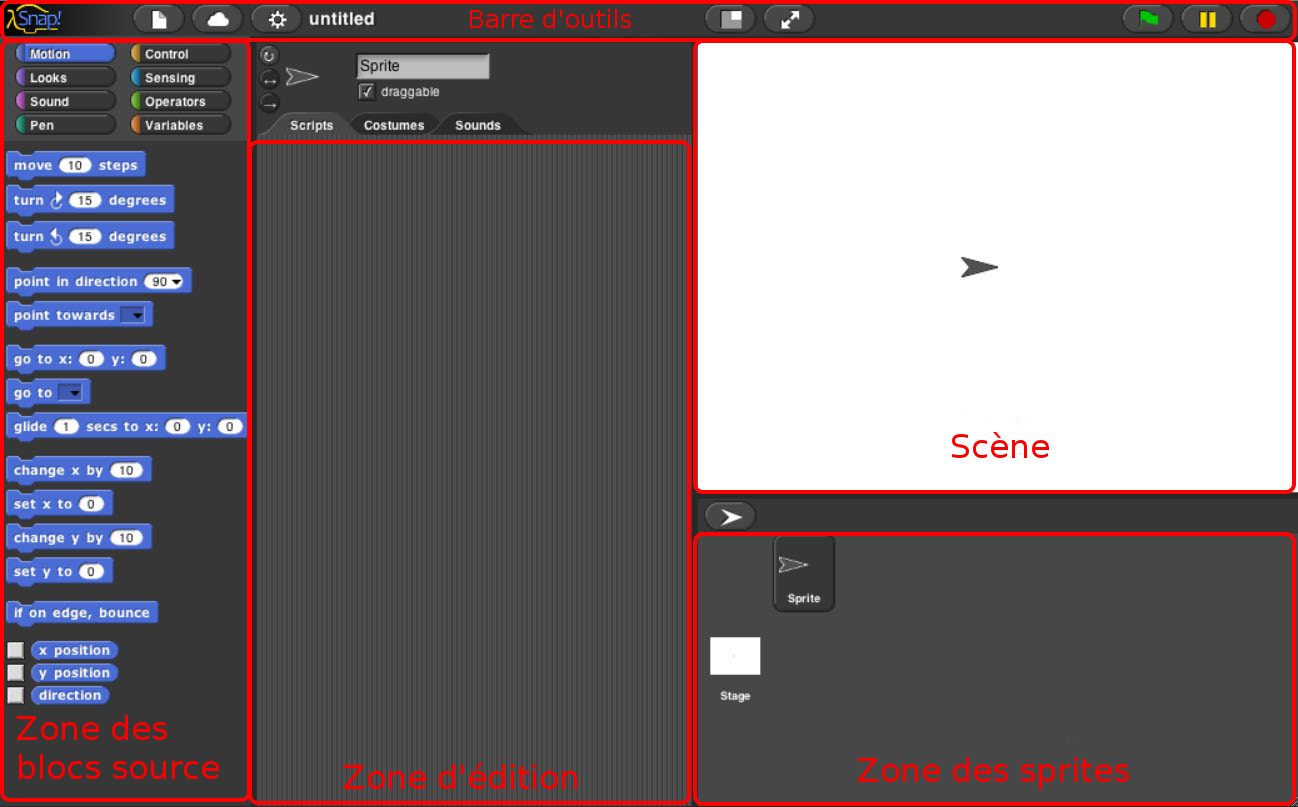
\includegraphics[width=\textwidth]{content/7-solution/2-snap/images/interface}
        \caption{Délimitation des zones de l'interface Snap!}
    \label{fig:snap interface}
  \end{center}
\end{figure}

\subsection{Blocs}
Il existe plusieurs types de \glspl{bloc} qui constituent un programme \gls{snap} \cite{snap-man}. Sur la figure \ref{fig:software-used-script}, le programme présente les différents types de \glspl{bloc} disponibles.
\begin{figure}
  \begin{center}
    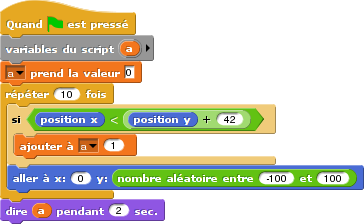
\includegraphics[width=0.5\textwidth]{content/5-related_work/images/script}
    \caption{Exemple de programme Snap!}
    \label{fig:software-used-script}
  \end{center}
\end{figure}

\subsubsection{Commande}
Le type principal de \glspl{bloc} est \texttt{commande}. Ces \glspl{bloc} peuvent être compris comme étant des procédures. En effet, ils exécutent une ou plusieurs opérations sur le système en fonction de paramètres fournis. Ces différents \glspl{bloc} doivent se baser soit sur une implémentation JavaScript pour les \texttt{commande}'s élémentaires, soit être une composition de \texttt{commande}'s pour fournir une nouvelle \texttt{commande} plus complexe ou abstraite.

Dans l'exemple de la figure \ref{fig:software-used-script}, tous les \glspl{bloc} \texttt{commande} ont la forme d'une pièce de puzzle. On peut y voir qu'une succession de \texttt{commande}'s crée un \gls{script}. Les \texttt{commande}'s ont plusieurs couleurs suivant la catégorie à laquelle elles appartiennent : mouvement, apparence, contrôle, variable \ldots

\subsubsection{Reporter}
Les \texttt{reporter}'s sont des fonctions. En effet, ils renvoient une valeur. Ils sont toujours utilisés en temps que paramètres d'un autre \gls{bloc}. La plupart des \texttt{reporter}'s sont des accesseurs à des variables ou à des états du système (position souris, heure \ldots).

Les \texttt{reporter}'s sont des \glspl{bloc} de forme arrondie. La figure \ref{fig:software-used-script} montre différentes utilisations de \texttt{reporter} : somme, valeur aléatoire, position, etc. Tout comme pour les \texttt{commande}'s, les \texttt{reporter}'s peuvent être de diverses couleurs suivant leur catégorie.

\subsubsection{Prédicat}
Les \texttt{predicat}'s sont des reporters qui retournent une valeur booléenne. Ils sont donc utilisés en conjonction avec des commandes demandant une condition. Les \texttt{predicat}'s ont une forme hexagonale.
%TODO ajouter un exemple

\subsubsection{Chapeau}
Les \texttt{hat}'s sont des commandes spéciales, car ils sont le point d'entrée obligatoire d'un \gls{script} en permettant de démarrer l'exécution de celui-ci. Plusieurs types d'événements peuvent lancer un \gls{script} : une touche pressée, un clic sur le drapeau vert etc.

Dans la figure \ref{fig:software-used-script}, le démarrage du programme est l'événement qui lance le \gls{script}. Il est symbolisé par un drapeau vert.

\subsection{Programme}
\gls{snap} est plus qu'une interface graphique permettant de construire un programme. L'analyse de son fonctionnement interne est l'objet de ce paragraphe.

Un programme est constitué de plusieurs processus. Chaque processus est exécuté en parallèle grâce à un ordonnanceur.

% /*
%     A Process is what brings a stack of blocks to life. The process
%     keeps track of which block to run next, evaluates block arguments,
%     handles control structures, and so forth.
%
%     The ThreadManager is the (passive) scheduler, telling each process
%     when to run by calling its runStep() method. The runStep() method
%     will execute some number of blocks, then voluntarily yield control
%     so that the ThreadManager can run another process.
%
%     The Scratch etiquette is that a process should yield control at the
%     end of every loop iteration, and while it is running a timed command
%     (e.g. "wait 5 secs") or a synchronous command (e.g. "broadcast xxx
%     and wait"). Since Snap also has lambda and custom blocks Snap adds
%     yields at the beginning of each non-atomic custom command block
%     execution, and - to let users escape infinite loops and recursion -
%     whenever the process runs into a timeout.
%
%     a Process runs for a receiver, i.e. a sprite or the stage or any
%     blocks-scriptable object that we'll introduce.
%
%     structure:
%
%     topBlock            the stack's first block, of which all others
%                         are children
%     receiver            object (sprite) to which the process applies,
%                         cached from the top block
%     context                the Context describing the current state
%                         of this process
%     homeContext            stores information relevant to the whole process,
%                         i.e. its receiver, result etc.
%     isPaused            boolean indicating whether to pause
%     readyToYield        boolean indicating whether to yield control to
%                         another process
%     readyToTerminate    boolean indicating whether the stop method has
%                         been called
%     isDead              boolean indicating a terminated clone process
%     timeout                msecs after which to force yield
%     lastYield            msecs when the process last yielded
%     errorFlag            boolean indicating whether an error was encountered
%     prompter            active instance of StagePrompterMorph
%     httpRequest         active instance of an HttpRequest or null
%     pauseOffset         msecs between the start of an interpolated operation
%                         and when the process was paused
% */

Un processus \texttt{Process} représente l'exécution d'un \gls{script}, une pile de \glspl{bloc}. Il assure aussi le suivi de l'exécution du \gls{script} : prochain \gls{bloc} à exécuter, objet sur lequel il s'applique, contexte décrivant l'état courant, etc.

L'ordonnanceur \texttt{ThreadManager} appelle la fonction \texttt{runStep()} (extrait de code source \ref{lst-runstep}) successivement sur chaque processus. Cette fonction exécute un certain nombre de \glspl{bloc} via \texttt{this.evaluateContext()} de manière atomique. Elle rend la main volontairement à l'ordonnanceur quand elle a fini. Comme il est possible d'écrire soi-même des \glspl{bloc}, \texttt{runStep()} rend aussi la main si trop de temps s'est écoulé depuis le début de l'exécution de cette étape. La convention veut que les processus rendent la main à la fin de chaque itération de boucle et quand une opération relative au temps ou synchrone est exécutée.
\begin{figure}
\begin{lstlisting}[caption={Fonction \texttt{runStep()} de \texttt{Process}},label=lst-runstep,language=JavaScript]
Process.prototype.runStep = function () {
/*
    a step is an an uninterruptable 'atom', it can consist
    of several contexts, even of several blocks
*/
    // allow pausing in between atomic steps:
    if (this.isPaused) {
        return this.pauseStep();
    }
    this.readyToYield = false;
    while (!this.readyToYield
            && this.context
            && (this.isAtomic ? (Date.now() - this.lastYield < this.timeout) : true) ) {
        // also allow pausing inside atomic steps - for PAUSE block primitive:
        if (this.isPaused) {
            return this.pauseStep();
        }
        this.evaluateContext();
    }
    this.lastYield = Date.now();

    // make sure to redraw atomic things
    if (this.isAtomic &&
            this.homeContext.receiver &&
            this.homeContext.receiver.endWarp) {
        this.homeContext.receiver.endWarp();
        this.homeContext.receiver.startWarp();
    }

    if (this.readyToTerminate) {
        while (this.context) {
            this.popContext();
        }
        // pen optimization
        if (this.homeContext.receiver &&
                this.homeContext.receiver.endWarp) {
            this.homeContext.receiver.endWarp();
        }
    }
};
\end{lstlisting}
\end{figure}


% /*
%     A Context describes the state of a Process.
%
%     Each Process has a pointer to a Context containing its
%     state. Whenever the Process yields control, its Context
%     tells it exactly where it left off.
%
%     structure:
%
%     parentContext    the Context to return to when this one has
%                     been evaluated.
%     outerContext    the Context holding my lexical scope
%     expression        SyntaxElementMorph, an array of blocks to evaluate,
%                     null or a String denoting a selector, e.g. 'doYield'
%     receiver        the object to which the expression applies, if any
%     variables        the current VariableFrame, if any
%     upvars          the current UpvarReference, if any (default: null)
%     inputs            an array of input values computed so far
%                     (if expression is a    BlockMorph)
%     pc                the index of the next block to evaluate
%                     (if expression is an array)
%     startTime        time when the context was first evaluated
%     startValue        initial value for interpolated operations
%     activeAudio     audio buffer for interpolated operations, don't persist
%     activeNote      audio oscillator for interpolated ops, don't persist
%     isLambda        marker for return ops
%     isImplicitLambda    marker for return ops
%     isCustomBlock   marker for return ops
%     emptySlots        caches the number of empty slots for reification
% */

\subsection{Interface graphique}
Un autre élément intéressant à analyser chez \gls{snap} est sa façon d'afficher l'interface dans la balise HTML \texttt{canvas} (voir code source \ref{lst-doonecycle}). Toutes les fonctionnalités nécessaires à afficher tous les éléments graphiques de \gls{snap} découlent de l'implémentation que l'on retrouve dans \texttt{morphic.js}.

\texttt{morphic.js} fournit les abstractions pour redessiner des parties de l'interface et pour interagir avec l'utilisateur. Le \texttt{canvas} utilisé possède un \texttt{world}. Ce \texttt{world} est la racine de l'arbre composé de \texttt{morph} et leurs sous-\texttt{morph}. Chaque \texttt{morph} peut être déplacé, redimensionné via le code source ou les manipulations de l'utilisateur.

La fonction principale de \texttt{morphic.js} consiste à parcourir continuellement tous les éléments du \texttt{world} pour redessiner ceux qui ont été modifiés. Le \texttt{world} permet à l'ordonnanceur d'exécuter une étape entre chaque itération. Le code source \ref{lst-doonecycle} montre que le \texttt{world} est rafraîchit toutes les 50 millisecondes.
\begin{figure}
\begin{lstlisting}[caption={Exemple d'utilisation de \texttt{morphic.js}},label=lst-doonecycle,language=HTML5,alsolanguage=JavaScript]
<!DOCTYPE html>
<html>
    <head>
        <title>Morphic!</title>
        <script type="text/javascript" src="morphic.js"></script>
        <script type="text/javascript">
            var world;

            window.onload = function () {
                world = new WorldMorph(
                    document.getElementById('world'));
                setInterval(loop, 50);
            };

            function loop() {
                world.doOneCycle();
            }
        </script>
    </head>
    <body>
        <canvas id="world" tabindex="1" width="800" height="600" />
    </body>
</html>
\end{lstlisting}
\end{figure}
La fonction \texttt{drawNew()} sert à dessiner un \texttt{morph}. Le code source \ref{lst-drawnew} montre que cette fonction dessine son objet sur une image stockée dans l'objet. Cette image provient d'un \texttt{canvas} virtuel généré grâce à l'image du \texttt{morph} parent.

\begin{figure}
\begin{lstlisting}[caption={Modèle pour la fonction \texttt{drawNew()}},label=lst-drawnew,language=JavaScript]
MyMorph.prototype.drawNew = function() {
    var context;
    this.image = newCanvas(this.extent());
    context = this.image.getContext('2d');
    // use context to paint stuff here
};
\end{lstlisting}
\end{figure}

\section{Ruby on Rails}
\label{rails}
\gls{rails} \cite{rails} est une plateforme de développement d'applications web basée sur le langage de programmation Ruby \cite{ruby}. Cette partie présente la philosophie, l'architecture et des environnements de tests de \gls{rails}.

\subsection{Philosophie}
\gls{rails} part de l'hypothèse qu'il existe une meilleure façon d'aborder la création d'applications web \cite{rails-guides}. Si le programmeur respecte ce "Rails way", il améliorera sa productivité et écrira moins de code. D'après \gls{rails}, s’il persiste à utiliser ses anciennes habitudes, le développeur s'amusera beaucoup moins en créant son application.

Pour atteindre cet objectif, \gls{rails} utilise deux principes majeurs :
\begin{description}
  \item[Convention plutôt que configuration (CoC) \cite{wiki-coc} :] Pour permettre au programmeur d'écrire moins de code, \gls{rails} permet de n'écrire que ce qui ne correspond pas aux conventions. \gls{rails} utilise la métaprogrammation pour fournir les conventions à tous les objets.
  \item[Ne vous répétez  pas (DRY) \cite{wiki-dry} :] \gls{rails} recommande une architecture où il faut mettre l'information à un endroit unique et bien déterminé. Ceci permet d'avoir un code plus court, plus maintenable, plus extensible et avec moins de bogues.
\end{description}

\label{rbp}
Un service aidant à mieux comprendre et respecter le "Rails way" est Rails\_best\_practices. Il fournit des métriques utiles pour détecter des écarts à la philosophie \gls{rails}. Cet outil s'utilise avec les conseils fournis par \url{http://rails-bestpractices.com} aidant à refactorer les morceaux de code qui ne respecteraient pas les conventions.

\subsection{Architecture}
\gls{rails} se base sur une architecture \gls{mvc} \cite{wiki-mvc} (figure \ref{fig:mvc}).
\begin{figure}[ht]
  \begin{center}
    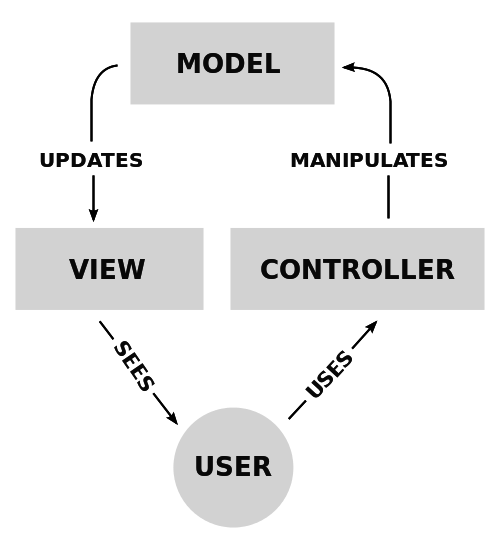
\includegraphics[scale=0.3]{content/4-prerequis/images/mvc}
    \caption{Schéma interaction d'un modèle MVC}
    \label{fig:mvc}
  \end{center}
\end{figure}
\subsubsection{Modèle}
Un modèle est typiquement une classe qui représente une table de la base de données. Une classe du modèle fournit aussi toutes les méthodes nécessaires à représenter et modifier l'objet dans le domaine d'application.

La correspondance entre un objet Ruby et la base de données est réalisée grâce à \textit{Active Record}. Ce module de \gls{rails} permet de faire des appels sur des objets Ruby alors que dans d'autres framework, il faudrait utiliser des requêtes \textit{SQL}. \label{active-record}

\subsubsection{Contrôleur}
\label{controleur}
Le contrôleur a pour fonction d'accéder à une ressource. Une ressource est un modèle ou tout autre objet indirect tel qu’enregistrement, login, page d'accueil\ldots

Il détermine quelle vue doit s'afficher et avec quels paramètres. Le contrôleur a donc la tâche de vérifier la sécurité et l'intégrité des données fournies par l'utilisateur. Ensuite, il peut interroger différents modèles et fournir les réponses à la vue adéquate.

\label{rest}\label{rails-routes}
\gls{rails} encourage à avoir des ressources \gls{rest} \cite{wiki-rest}, c'est-à-dire, des ressources avec une représentation unique et des actions unifiées telles que create, new, edit, update, destroy, show, index. Les actions disponibles sur un contrôleur sont déterminées par le fichier de configuration des routes.

\subsubsection{Vue}
Les vues correspondent à ce que les utilisateurs reçoivent et voient. Ce sont typiquement des pages HTML, mais aussi des PDF, objets JSON, fichiers, etc

Pour faciliter la création des vues, \gls{rails} permet d'utiliser des \glspl{gem}. Il existe notamment:
\begin{description}
  \item[Haml \cite{haml} \label{haml} :] un langage fournissant une syntaxe raccourcie du HTML. Il se base sur l'indentation plutôt que sur une syntaxe XML. Haml permet donc de respecter le principe \texttt{DRY} et d'améliorer la lisibilité par un code source plus court et bien indenté ;
  \item[JQuery \cite{jquery} :] cette bibliothèque JavaScript bien connue permet de modifier facilement le document courant, de gérer des événements, de créer des animations, etc. ;
  \item[CoffeeScript \cite{coffeescript} :] est un langage qui se compile en JavaScript. Il permet d'avoir une syntaxe plus claire, plus courte et d'ajouter des sucres syntaxiques par rapport à JavaScript;
  \item[Bootstrap \cite{bootstrap} :] est un framework CSS qui découple le fond et la forme de l'affichage d'une page HTML. Ce framework donne un design adaptatif pour tous types d'écrans aux pages qui l'utilisent. Il fournit aussi de nombreux composants utiles : boutons, alertes, barres de progression, messages d'aide, etc. \label{bootstrap}
\end{description}
%TODO intégré avec les contrôleurs. Paperclip dans les vues
\subsection{Gems}
\label{gems}
Ruby fournit une manière de partager des fonctionnalités pour des programmes Ruby via les \glspl{gem} \cite{gem}. \gls{rails} lui-même est un \gls{gem} et dépend de nombreux autres notamment Active Record présenté plus haut.

\label{gemnasium}
La communauté de \gls{rails} a écrit de nombreux \glspl{gem}  permettant de rajouter facilement des fonctionnalités à une application. Le fichier \texttt{Gemfile} sert à lister les \glspl{gem}  utilisés dans un projet. Le gestionnaire du projet doit faire attention à toutes ces dépendances pour garder son logiciel à jour. Pour ce faire, Gemnasium analyse le fichier \texttt{Gemfile} pour indiquer quels \glspl{gem}  doivent être mis à jour. Gemnasium informe donc les gestionnaires d'un logiciel lorsqu'une faille de sécurité est découverte dans un \gls{gem} et qu'il faut donc le mettre à jour.

Quelque exemples de \glspl{gem} intéressants sont présentés ci-après.
\begin{description}
  \item[Paperclip \cite{paperclip} :] permet de facilement récupérer et stocker des fichiers. Paperclip intègre donc la gestion de fichiers tiers de manière élégante dans une classe du modèle. Il fournit notamment divers pilotes pour stocker ces fichiers aussi bien en local que sur le nuage d'Amazon ou de Dropbox.
  \item[Devise \cite{devise} :] gère la problématique de l'authentification des utilisateurs.
  \item[Rolify \cite{rolify} :] donne des \glspl{role} aux utilisateurs de manière générale (ex. administrateur) ou sur une ressource (ex. modérateur d'un forum).\label{rolify}
  \item[Authority \cite{authority} :] gère les droits des utilisateurs sur les différentes ressources des contrôleurs. \label{authority}
\end{description}

\subsection{Tests}
\label{rails-tests}
Il existe tout un écosystème autour de \gls{rails} pour fournir du code de qualité. Cette partie présente quelques outils utilisés dans les tests. Les outils les plus employés sont présentés ci-dessous, bien que ce ne soit pas les seuls existants.

\subsubsection{Tests comportementaux}
\label{cucumber}
Un outil de test fort apprécié des programmeurs Ruby et plus particulièrement \gls{rails} est Cucumber \cite{cucumber}. Ce dernier réalise des tests dans un "behavior-driven development" \cite{wiki-bdd} style. Ce style de tests se compose de deux parties. D'une part, le client ou chef de projet écrit des scénarii qui décrivent l'utilisation de fonctionnalités du domaine en langage naturel (Gherkin \cite{gherkin}). D'autre part, le programmeur implémente ces scénarii. Ce type de test met l'accent sur ce que voit le client. Si tout ce que voit le client fonctionne, c'est que le coeur utile de l'application est correct.

Dans le cas de \gls{rails}, il est intéressant d'utiliser conjointement Cucumber et Capybara \cite{capybara}. Ce dernier permet de contrôler un navigateur et donc de réaliser des tests à la place d'un utilisateur. Ces tests permettront d'assurer le bon fonctionnement de ce que souhaite l'utilisateur.

\subsubsection{Intégration continue}
\label{travis}
Dans le cadre d'un développement actif, il est intéressant d'avoir un serveur qui réalise des tests d'intégration continue \cite{wiki-int-cont}. En effectuant les tests lors de chaque nouveau \texttt{commit}, les développeurs sont informés directement si une modification du code source a induit une régression des fonctionnalités. Ce service est proposé, entre autres, par \texttt{Travis CI}\cite{travis}.


\chapter{Travaux associés}
\label{travail associé}
Cette partie présente ce qui se fait déjà dans le monde à l'heure actuelle en matière d'apprentissage de la programmation.

Premièrement, il y aura un tour d'horizon des politiques gouvernementales de pays qui ont adopté l'apprentissage de la programmation dans leur programme officiel. Ceci présentera les avancées de cette problématique et aidera à envisager différentes manières de la traiter. 

Après ce tour d'horizon, l'attention sera portée sur des organisations non gouvernementales qui ont pour but de promouvoir l'enseignement de la programmation. 

La troisième partie décrira les langages utilisés dans les organisations présentées précédemment. 

Enfin, des concepts différenciateurs seront extraits de chaque initiative afin les distinguer l'une de l'autre.
\section{État de la programmation dans le monde}
\label{monde} %TODO dire pourquoi la politique influe sur la problématique
Cette section fait un tour d'horizon de différents pays qui enseignent la programmation aux jeunes. L'accent est mis spécialement sur leur positionnement politique et leur manière d'intégrer l'apprentissage de la programmation.
\subsection{Angleterre}
L'apprentissage de l'informatique en Angleterre\footnote{\url{https://www.gov.uk/government/collections/statutory-guidance-schools\#national-curriculum-from-september-2014}} n'est pas nouveau. Pendant longtemps, il était centré sur les technologies de l'information et de la communication (TIC). C'est donc principalement l'utilisation de l'informatique, et non sa conception qui était enseignée.

En 2010, une étude a été commandée à la Royal Society pour évaluer cet apprentissage. Un an plus tard, le rapport a révélé que l'enseignement n'est ni efficace ni en adéquation avec l'évolution de l'informatique dans leur société. La Royal Society suggère d'adapter les matières abordées en informatique en enseignant l'apprentissage de la programmation. Sur base de ce rapport, les programmes de cours ont été modifiés en 2012.

\subsection{France}
En France\footnote{\url{http://fr.wikipedia.org/wiki/Informatique\_et\_sciences\_du\_num\%C3\%A9rique}
\url{http://fr.wikipedia.org/wiki/Baccalaur\%C3\%A9at\_scientifique}}, depuis deux ans, l'informatique fait partie intégrante du programme du baccalauréat de type S. Une des matières dispensées est "Informatique et sciences du numérique". Cette matière se subdivise en quatre sous parties : représentation de l'information, algorithmique, langage et programmation, architectures matérielles. Cette approche est donc également basée sur l'apprentissage de la programmation plutôt que sur les TIC.

\subsection{Corée du Sud}
La Corée du Sud enseigne l'informatique depuis longtemps et à tous les niveaux de l'enseignement. La culture numérique dans les pays asiatiques est fort différente de ce que l'on connait chez nous. Par exemple, une carrière dans le jeu vidéo est quelque chose de tout à fait normal. L'informatique est vraiment omniprésente dans cette culture, il est donc normal que son apprentissage commence dès l'enseignement fondamental.

\subsection{Grèce}
L'apprentissage des sciences informatiques prend une place importante dans les programmes grecs. Dès 6 ans, les enfants sont confrontés à l'informatique à l'école. À cet âge, ils apprennent principalement la maîtrise de l'outil. Dès 10 ans, leurs cours d'informatique prennent une tournure plus algorithmique et donc plus proche de la science de l'informatique.

\subsection{Nouvelle-Zélande}
Ce pays a adopté récemment les sciences informatiques dans son programme d'étude. Les cours sont dispensés à partir de 15 ans. Ces cours comprennent l'apprentissage de la programmation et de concepts informatiques en général. La nouvelle-Zélande, en introduisant les cours tardivement, s'inscrit dans une logique similaire à la France sans toute fois restreindre l'informatique aux options scientifiques.

\subsection{La belgique \ldots}
%TODO to be 
L'apprentissage de la programmation est déjà bien avancé dans plusieurs pays. Ce n'est malheureusement pas encore tout à fait le cas dans le nôtre. En effet, quelques initiatives locales existent, mais aucune décision politique n'a été prise jusqu'à présent.\\
\section{Organisations existantes}
Il sera présenté ici un ensemble d'initiatives à ce travail qui s'inscrivent la logique de ce travail. Elles sont toutes non gouvernementales et proposent d'enseigner la programmation de différentes manières.
\subsection{Code.org}
\begin{figure}[!ht]
  \begin{center}
    
\includegraphics[scale=0.5]{content/5-related_work/images/code}
    \caption{Logo de code.org}
    \label{fig:code.org}
  \end{center}
\end{figure}
Code.org \cite{code-org-about} est une organisation sans but lucratif des USA qui a pour objectifs :
\begin{itemize}
  \item apporter l'informatique dans toutes les classes de \gls{secondaire} aux États-Unis ;
  \item démontrer le succès de l'utilisation de cours en ligne dans l'enseignement public ;
  \item ajouter l'informatique dans les bases des programmes de sciences et de mathématique des 50 états ;
  \item employer la connaissance technique collective pour améliorer l'apprentissage de l'informatique dans le monde ;
  \item augmenter la représentation féminine et de personnes de couleurs dans l'informatique.
\end{itemize}

Pour ce faire, Code.org fournit une plate-forme \cite{code-org-20hr} web qui permet aux professeurs de suivre leurs élèves grâce à un système de classes. Ce programme d'apprentissage se base sur Blockly (voir \ref{blockly}).

Toutes les ressources sont gratuites et librement utilisables \cite{code-org-faq}. Elles sont conçues pour que les professeurs comme les élèves puissent commencer le cours sans connaître l'informatique (une assistance gratuite est proposée au professeur si nécessaire).

Le site propose aux professeurs de se faire récompenser s'ils arrivent à finir les 27 \glspl{mission} proposées avec minimum 15 élèves. Dans ce cas, ils gagnent $750\$$. S'ils ont au moins 7 filles dans le groupe, ils peuvent prétendre à $250\$$ supplémentaires.

\subsubsection{Déroulement des leçons}
Code.org propose des sessions d'une heure de travail/jeu/apprentissage. Chaque unité est découpée en \glspl{mission} courtes (ex:5-20) apportant un concept de programmation. Avant chaque concept, une petite vidéo l'introduit et donne des exemples d'utilisation.

Il propose de faire travailler les élèves en binôme \cite{wiki-pair-prog}, ce qui entraîne moins de questions au professeur et permet de mieux s'approprier la matière. Le travail par binôme casse également l'image du "geek" et montre que la programmation est une science sociale et collaborative. De plus, moins d'ordinateurs sont nécessaires.

Le site explique également que pour faire participer tous les élèves, il faut avoir confiance en leurs compétences. La philosophie est d'inciter les premiers groupes à aider les derniers.

Quand un élève a une question, Code.org recommande de la soumettre à 3 de ses camarades avant de la poser au professeur. Cela permet aussi d'éviter les questions de distraction ou de manque de compréhension.

Pour chaque petite \gls{mission}, un test automatisé informe si la \gls{mission} est réussie ou non. Si celle-ci est réussie, la plateforme propose la \gls{mission} suivante. Dans les premières \glspl{mission}, il y a également un compteur de \glspl{bloc} qui informe du nombre de \glspl{bloc} nécessaires pour réaliser la \gls{mission} de manière optimale.

\subsection{CoderDojo}
\begin{figure}[!ht]
  \begin{center}
    
\includegraphics[scale=0.5]{content/5-related_work/images/dojo}
    \caption{Logo de CoderDojo}
    \label{fig:coder dojo}
  \end{center}
\end{figure}
CoderDojo \cite{dojo-about} est un réseau open source de Clubs de programmation dans le sens le plus large du terme. Tous les dojos sont donc autonomes. Des enfants de 5 à 17 ans y apprennent la programmation (site web, application, jeux...). La seul règle est "Above All : Be Cool" qui est mise en pratique en créant simplement des espaces d'échanges de savoirs amicaux et sociables.

CoderDojo a été créé par James Whelton, un irlandais de 18 ans, et Bill Liao, un entrepreneur australien à Cork. James, après avoir hacké l'iPod nano, a eu des demandes de jeunes enfants pour avoir des cours de programmation. Beaucoup de gens de Dublin ont été à ses cours et donc un nouveau Dojo y a été créé. Ensuite, cela s'est étendu à tout le globe.

\subsection{Code Club}
\begin{figure}[H]
  \begin{center}
    
\includegraphics[scale=0.3]{content/5-related_work/images/club}
    \caption{Logo de Code Club}
    \label{fig:code club}
  \end{center}
\end{figure}
Code Club\cite{codeclub-about} est un réseau national de Clubs mené par des bénévoles en dehors des heures de cours. Leurs activités s'adressent à des enfants de 9 à 11 ans.

Ils créent le matériel pour permettre à des bénévoles de donner des cours parascolaires d'environ une heure par semaine. Ils proposent d'utiliser dans cet ordre scratch, HTML/css et puis Python. Ils ont pour objectif que les 21000 écoles \glspl{fondamental} anglaises aient leur club.

Leur philosophie est de favoriser l'amusement, la créativité et l'exploration avant l'apprentissage des concepts de programmation.

\subsection{KidsCode}
\label{init-kidscode}
\begin{figure}[!ht]
  \begin{center}
    
\includegraphics[scale=0.5]{content/5-related_work/images/kidscode}
    \caption{Logo de KidsCode}
    \label{fig:kidscode}
  \end{center}
\end{figure}
KidsCode \cite{kidscode} est une petite initiative wallonne qui organise actuellement un stage pour les enfants de 10 à 14 ans. Les ateliers sont dispensés par deux informaticiens qui proposent de partager leur passion. Ils encadrent les jeunes de manière ludique dans le but de les rendre autonomes.

KidsCode propose d'apprendre la programmation grâce au langage Python. Ce langage a été choisi pour sa facilité tout comme pour son utilisation en condition réelle.

KidsCode a été conçu et pensé en association avec l'incubateur de startup Nestup. Cette initiative est le fruit du constat par les entreprises, d'un manque d'intérêt pour la programmation chez les plus jeunes. Ceci entraîne un manque de vocations dans les startups.

\section{Langages de programmation}
\label{langages}
Cette partie traite des différents éditeurs et langages de programmation utilisés dans les organisations présentées au point précédent.

\subsection{Blockly}
\label{blockly}

\begin{figure}[!ht]
  \begin{center}
    
\includegraphics[scale=0.5]{content/5-related_work/images/blocky}
    \caption{Logo de Blocky}
    \label{fig:blocky}
  \end{center}
\end{figure}
Blockly \cite{blockly} est un langage de programmation graphique basé sur des technologies du web.

Blockly a comme particularité :
\begin{itemize}
\item de s'exécuter dans un navigateur ;
\item d'exporter du code source en JavaScript, Dart, etc. ;
\item d'être open source ;
\item d'être haut niveau.
\end{itemize}

Il n'est pas directement une plateforme d'éducation dans le sens où, il peut être utilisé autant pour l'éducation, le business, des jeux, \ldots en fonction des \glspl{bloc} implémentés.\\

Blockly a été conçu avec certaines propriétés choisie lors de sa création. Les trois premières augmentent la compréhension des néophytes, les autres portent sur des facilités du langage. Les propriétés décidées lors de la conception du langage sont \cite{blockly-lang} :

\begin{itemize}
  \item des indices de listes commençant à 1 ;
  \item des noms de variables non sensibles à la casse ;
  \item pas de portée de variable, elles sont toutes globales ;
  \item la possibilité de faire un export en JavaScript ;
  \item un code natif généré proche de celui des \glspl{bloc}.
\end{itemize}

\subsection{Scratch}

\begin{figure}[!ht]
  \begin{center}
    
\includegraphics[scale=0.4]{content/5-related_work/images/scratch}
    \caption{Logo de Scratch}
    \label{fig:scratch}
  \end{center}
\end{figure}
Scratch \cite{scratch} est un langage de programmation graphique développé par le MIT pour apprendre aux enfants la programmation. C'est l'interface qui permet de faire des scripts facilement grâce à une programmation par \glspl{bloc} et du glisser-déposer.\\

Il a été pensé pour être un outil créatif pour réaliser des histoires, des jeux, des simulations, de l'art, etc. Il a, par exemple, son propre éditeur d'image et de sons. Un autre but de ce langage est d'être simple à utiliser et à apprendre. Il a en effet été conçu pour des enfants n'ayant aucune connaissance préalable en programmation.\\

Actuellement Scratch est à sa version 2 qui est une version web. Cette version a été complètement réécrite en flash par rapport à la version 1 en Smalltalk. De plus, la version 2 n'est plus open source contrairement à la première version.

Comme le montre la figure \ref{fig:scratch-printscreen}, l'interface de Scratch se divise en plusieurs grandes parties :

\begin{enumerate}
\item sur la gauche, il y a la zone de dessin dans laquelle s'anime les composants graphiques des scripts ;
\item au milieu, une liste des \glspl{bloc} disponible triés par catégorie ;
\item sur la droite, la zone de script qui contient tous les scripts liés au sprite sélectionné.
\end{enumerate}

\begin{figure}
  \begin{center}
    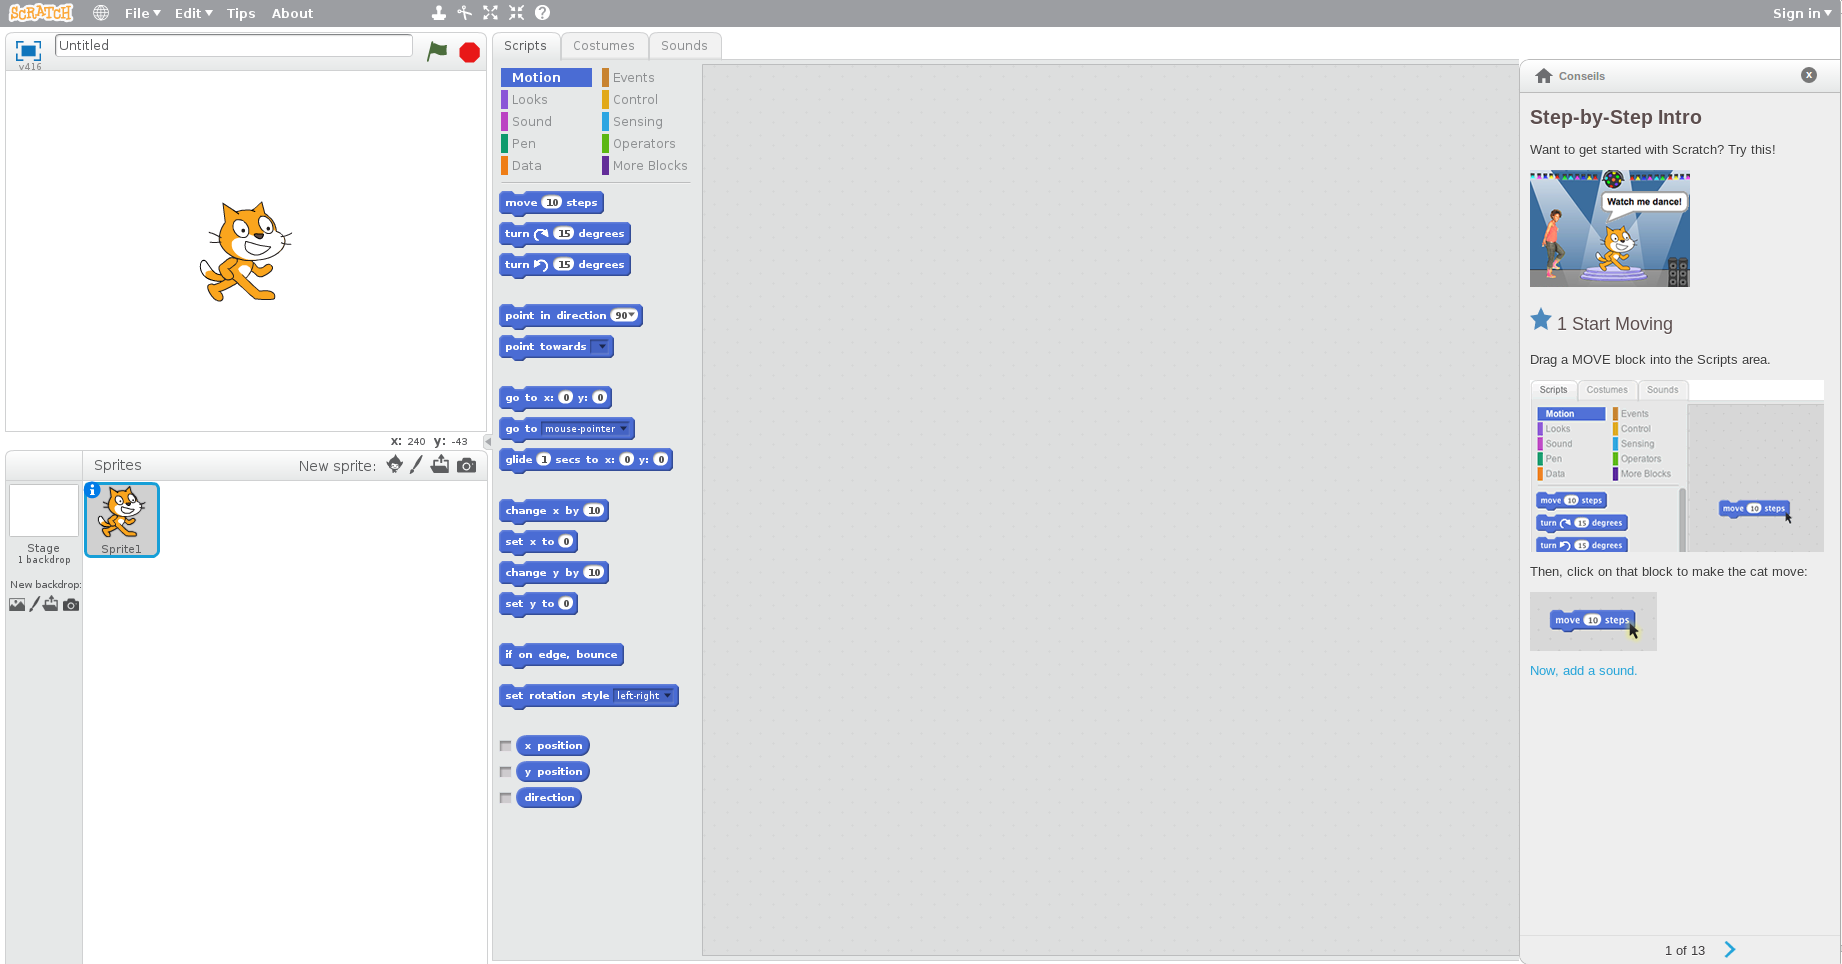
\includegraphics[width=\textwidth]{content/5-related_work/images/scratch-printscreen}
    \caption{Interface de Scratch}
    \label{fig:scratch-printscreen}
  \end{center}
\end{figure}

\subsection{Snap!}

\begin{figure}[!ht]
  \begin{center}
    
\includegraphics[scale=0.07]{content/5-related_work/images/snap}
    \caption{Logo de Snap!}
    \label{fig:snap}
  \end{center}
\end{figure}

Snap! \cite{snap} est un langage de programmation de "glissé-déposé" de \glspl{bloc}. C'est une ré-implémentation et une extension du langage Scratch du MIT. Il a été pensé et conçu pour être orienté web. Il est donc implémenté en JavaScript.\\

Ce langage est né en 2011 et a été créé par Jens Mönig, docteur de l'université de Berkeley. Il se distingue de son père Scratch par l'ajout :
\begin{enumerate}
\item fonctions et procédures de première classe. Une entité dite de première classe est une entité qui supporte toutes les opération disponible sur d'autres entités ; %TODO glossaire premiere classe
\item listes de première classe ;
\item sprite de première classe.
\end{enumerate}

\subsection{Python}

\begin{figure}[!ht]
  \begin{center}
    
\includegraphics[scale=0.4]{content/5-related_work/images/python}
    \caption{Logo de Python}
    \label{fig:python}
  \end{center}
\end{figure}

Python \cite{python} est un langage de programmation qu'il ne faut plus présenter. Il a beaucoup d'avantages dont celui d'avoir une syntaxe légère et d'être facile à prendre en main. Une grande communauté et beaucoup de bibliothèques, dont la fameuse \texttt{turtle}, en fait un excellent langage pour démarrer dans la programmation.

Cependant, devoir apprendre un langage de programmation et la logique informatique en même temps complique la tâche. De plus, lorsqu'on commence un nouveau langage de programmation il faut également apprendre ses bonnes pratiques de codage. %TODO retravailler pour etre neutre

C'est donc un langage qui ne convient pas aux trop jeunes ni à ceux qui ne sont pas vraiment investis dans l'apprentissage de la programmation.

\section{Concepts différenciateurs}
\label{concepts}
Ce chapitre va mettre en lumière les différences et similitudes des méthodes d'apprentissage de la programmation en utilisant à une série de critères tels que le public cible, les moyens, le lieu et les personnes.
\subsection{Pour qui ?}
L'apprentissage de la programmation aux enfants est différenciée sur base de plusieurs critères tels que l'âge, l'origine, la classe sociale, le genre, etc. Les organisations auront donc soit un public visé restreint soit différents programmes pour les groupes d'enfants.

\subsubsection{Âge}
La méthode d'apprentissages doit être différente suivant l'âge. Les enfants n'ont pas tous la maturité pour apprendre des concepts abstraits (boucle, parallélisation...). Par exemple, pour des élèves de maternel, un tableau interactif sera un grand plus car ils n'ont pas encore la dextérité souhaitée pour manipuler la souris. Et au contraire, des enfants plus grands seront plus autonomes et pourront travailler par binôme voir seuls.

\subsubsection{Genre et origine}
Certaines organisations, telle Code.org, mettent l'accent sur la accessibilité pour tous en incitant à la participation des filles qui sont sous-représentées en informatique.

Les personnes qui ne peuvent acquérir un ordinateur ou se payer un stage ne doivent pas être délaissées.

\subsection{Comment ?}
Les principales différences entre toutes les organisations se situent dans la manière d'aborder l'apprentissage. Elles peuvent être de plusieurs ordres, tels que : les outils utilisés, les concepts abordés et l'environnement de travail.

\subsubsection{Outils}
Un aspect pratique qui différencie les apprentissages est le type de langage utilisé. Ici encore différentes écoles s'affrontent.

\paragraph{Le langage réel} Avec ce type de langage, les enfant apprennent la programmation et le langage utilisé. Ces langages sont plus difficiles à prendre en mains mais permette plus d'applications concrètes.
\paragraph{Le langage visuel} Dans la programmation, le plus important est la logique. Un langage qui se rapproche des diagramme allège la syntaxe, par exemple avec un langage de programmation par \glspl{bloc}.
\paragraph{Le langage web} Dans le monde d'aujourd'hui, le web est partout. L'accent doit donc être porté sur l'apprentissage de ce que les enfants voient au quotidien.


\subsubsection{Concepts}
Tous les cours se divisent en deux parties : la théorie et la pratique. Il existe de multiples manières d'assembler les deux dans un cours unique. L'ordre dans lequel les concepts de programmation sont abordés peut se différencier sur plusieurs points:
\begin{itemize}
  \item certains cours commencent par la théorie et demandent ensuite de l'appliquer ;
  \item d'autres proposent des exercices avant d'expliquer ce que les enfants ont utilisé de manière intuitive ;
  \item d'autres encore découpent la matière en petits sous-ensembles avant d'appliquer la première ou la seconde technique.\\
\end{itemize}


Ces différentes façons d'aborder l'apprentissage mènent diverses conceptions de \glspl{mission}. Celles-ci peuvent être très denses ou au contraire une succession de \glspl{mission} simples. Les \glspl{mission} denses sont souvent constituées de nombreux concepts de programmation (boucle, condition, fonction...) pour avoir directement un objectif concret alors que les \glspl{mission} simples essayent de bien séparer l'apprentissage pour fournir une étude la plus progressive possible.\\

Dans certains pays, la programmation est associée aux cours de sciences. Elle devient alors un outil qui perd du même coup une partie de son côté ludique. Par contre, elle touche un plus grand nombre d'enfants.\\

\subsubsection{Environement de travail}
\label{paire}
Les leçons peuvent être organisées de différentes manières :
\begin{description}
  \item[En groupe] L'apprentissage en groupe est souvent réalisé avec un tableau interactif ou un projecteur \footnote{\url{http://scratched.media.mit.edu/resources/scratch-\%C3\%A0-la-maternelle}} ;
  \item[Par binôme] La programmation en binôme est la plus répandue. Faire travailler les enfants par deux les oblige à interagir entre eux et à essayer de résoudre eux-mêmes les problèmes qu'ils rencontrent. Cela permet aussi de diminuer le nombre d'ordinateurs utilisés ;
  \item[Individuel] Cette technique est très peu utilisé, car elle demande beaucoup de moyens matériels et personnels. De plus, lors d'un apprentissage individuel, les étudiants se retrouve vite coincé et demande de l'aide ;
  \item[A domicile] De nombreuses plateformes proposent des cours en ligne qui peuvent être suivis au rythme de chacun. Néanmoins, pour avoir de l'aide, il faut se tourner vers une personne compétente ou vers les forums. Ces formations sont souvent plus théoriques et demandent plus de lecture, ce qui empêche les jeunes enfants de les suivre.
\end{description}

\subsection{De qui ?}
Chaque initiative s'organise suivant différents critères tels que l'intégration ou non dans un programme scolaire, les compétences des encadrants et le système de gestion des ressources

\subsubsection{Type d'organisation}
Les cours d'informatique sont soit donnés dans le cadre d'un programme officiel soit en parascolaire.

Dans le premier cas, les étudiants ne viennent pas tous par choix. Ceci peut entraîner entre autres des blocages et des réticences à participer correctement à l'activité.

Pour les cours donnés en parascolaire, des petites structures très locales se partagent le terrain avec de grandes organisations à visées internationales. Le coût des activités et les horaires en sont les problèmes typiques.

\subsubsection{Encadrants}
La plupart des cours sont donnés par des informaticiens ou au minimum des personnes formées à l'informatique. Mais comme le nombre d'informaticiens est réduit, certaines organisations proposent des cours clés-en-main pour des encadrants sans connaissance particulière en programmation. Ces professeurs apprennent en même temps que leurs étudiants et les aident à réfléchir.\\

Le type de rémunération des encadrants est assez diversifiée. Certains reçoivent des primes en fonction de la réussite de leur classe, d'autres sont payés par l'état ou directement par les étudiants, d'autres encore sont bénévoles.

\subsubsection{Gestion des ressources}
Suivant l'organisation, les cours sont plus ou moins figés. Certaines permettent à leur communauté de créer et/ou de modifier des cours tandis que d'autres ont des équipes dédiées à cette tâche.


\chapter{Définition de la problématique}
Ce chapitre a pour but de situer Rsnap par rapport aux initiatives similaires. Premièrement, Rsnap est positionné en reprenant les concepts différenciateurs du chapitre précédent \ref{concepts}. Ensuite, les besoins que la plateforme doit remplir sont abordés. Le troisième chapitre traite des choix technologiques qui ont été pris dans le cadre de ce travail.

\section{Positionnement de Rsnap}
\label{positionnement}
%XXX essais 1 (simon) pas beaucoup mieux que le précédent mais différent
Rsnap est la solution créée pour ce travail. Elle est conçue pour être l'outil privilégié pour faire interagir les professeurs avec leur élèves dans l'apprentissage de la programmation.
Cette première partie du chapitre présente qui, comment et grâce à qui est utilisé Rsnap.


% Rsnap veut combler des lacunes mises en évidence dans l'approche internationale \ref{monde}. En effet, aucune plateforme  web n'est disponible en français et peu se veulent orientées vers les professeurs. Sur le plan du langage, la plateforme Rsnap se veut entièrement en français pour pouvoir être utilisée par tous les enfants qui savent lire et étant inscrits dans l'enseignement francophone. Rsnap se veut aussi tourné vers les professeurs. Cela se traduit par une aide à la gestion de classe, une indépendance des enfants par rapport à un référent, l'absence de prérequis pour le professeur et l'édition de missions communautaires.\\
% 
% La suite de ce chapitre reprend les concepts abordés dans le chapitre \ref{concepts} et y positionne Rsnap.

\subsection{Âge, genre et origine des utilisateurs}
Le positionnement RSnap vis à vis de son public visé est présenté dans cette section.

\paragraph{Âge}
Rsnap se veut une application qui vise un public de 10 à 14 ans. Les missions qui ont été développées dans le cadre de ce travail ciblent particulièrement cette tranche d'âge. Cette question est nuancée par l'analyse des résultats des expérimentations abordée dans le chapitre \ref{trancheage}.
Toute fois, l'application permettant la création de mission de manière autonome, d'autres tranches d'âge peuvent s'y appliquer. La créativité des utilisateurs est la seule limite formelle.

\paragraph{Origine et genre}
En ce qui concerne les particularités des utilisateurs, aucune discrimination dans quelque sens que ce soit n'a été faite lors de la conception de ce travail, tant pour attirer un public que pour l'exclure. 

Comme l'idée est de proposer l'application dans les écoles de la Fédération Wallonie-Bruxelles, elle a été pensée pour un public francophone. 

\subsection{Outils, concepts et environnement de travail}
Cette section explique comment sont utilisés les différentes ressources pour apprendre la programmation aux enfants.

\paragraph{Outils}
\label{outil}
L'apprentissage de la programmation dans le but d'améliorer l'esprit logique des jeunes est un des objectifs principaux de ce travail. Dans cette optique, Rsnap se base sur un langage visuel \ref{langages}. L'accent est mis sur l'acquisition d'un esprit logique grâce à des exercices de logiques plutôt que sur l'apprentissage d'un langage de programmation.  En effet, suivant l'adage "il faut diviser pour mieux régner", vouloir tout faire en même temps ne convient pas à tous. En se concentrant sur la logique, cela assure une meilleure acquisition de la matière. De plus, un des buts de l'application Rsnap est aussi de susciter des vocations en programmation, ce qui se fera naturellement.

Un des objectifs de ce travail vise à ce que les personnes qui guident l'activité n'aient pas besoin de connaissance particulière en programmation. Un vrai langage de programmation a été écarté, car les encadrants auraient dû au minimum avoir connaissance de sa syntaxe.

\paragraph{Concepts}
La manière dont les concepts sont abordés dans Rsnap se fait par la procédure suivante :
\begin{itemize}
	\item une vidéo d'introduction à la mission ;
	\item un texte descriptif de la mission qui reprend les concepts théoriques introduits dans celle-ci ;
	\item une fois dans le programme, les jeunes n'ont plus d'explication explicite, ce qui les incite à travailler avec leur intuition tout en pouvant, si nécessaire, récupérer la description du point 2 ;
	\item une page d'aide est disponible pour chaque bloc dans le menu contextuel.
\end{itemize}

Les missions implémentées dans ce travail sont de petites missions introduisant un à deux grands concepts maximum. Ces petites missions ont pour but d'être assemblées pour faire un programme final plus important. Plus d'informations à propos du découpage et du contenu des missions sont disponibles dans la section \ref{missions}.

\paragraph{environnement de ce travail}
L'environnement de ce travail est déterminé prioritairement par son milieu d'utilisation, à savoir les écoles. 

L'indépendance des jeunes par rapport au référent oriente l'activité vers la formation de binôme. Toute fois, comme le groupe animé est une classe, une introduction collective est possible et souhaitable. 
Si les jeunes le souhaite, ils peuvent également avoir accès au site web en dehors du cadre scolaire.

\subsection{Type d'organisation, enseignants, création des cours}
Cette dernière section explique comment se positionne Rsnap par rapport aux personnes qui créeront les missions.

\paragraph{Type d'organisation}
Il n'y a pas d'organisation officielle qui supporte Rsnap. Elle pourrait être soit reprise par le gouvernement, soit être indépendante mais travailler pour ce dernier.

\paragraph{Enseignants}
À propos des enseignants, le projet a été créé dans le but que la personne qui dispense l'activité n'ait pas besoin de connaissance spécifique en programmation. Le simple fait de réaliser les projets avant les jeunes devrait être suffisant pour acquérir la logique nécessaire à la transmettre.

\paragraph{Création des cours}
La création des cours est un point sur lequel Rsnap se distingue de beaucoup d'autres. En effet, une partie des missions existent déjà et est intégrée à ce travail. Les professeurs peuvent également créer des missions et les partager avec le reste de la communauté. Tout comme ils peuvent aussi reprendre des missions existantes et les améliorer ou les adapter.

\section{Choix technologiques} %TODO revoir l'intro
\label{techno}
Pour mettre en pratique les concepts du chapitre précédent, des critères d'utilisation ont du être déterminés. La première partie a pour but de les présenter.

Ensuite, deux principales fonctionnalités sont abordées. %TODO oui je sais c'est de nouveau trop court ;)
D'une part, une une plateforme pour aider les professeurs à gérer leurs classes. Et d'autre part, un langage de programmation utilisé pour les missions d'apprentissage. 
% La nécessité d'une plateforme légère et accessible partout, pour ne pas dépendre du matériel propre aux écoles, oriente le choix vers une plateforme web.
% Comme introduite dans le chapitre \ref{rails}, la technologie Rails convient. La suite de ce chapitre développe les besoins et choix techniques pris pour le développement de cette plateforme. 

% Comme expliqué au chapitre \ref{SNAP}, le choix du langage de programmation s'est porté sur SNAP! BYOB. Comme cette application existait déjà, il va donc falloir l'intégrer à la plateforme web. Ce sera le dernier point développé.



\subsection{Analyse des besoins}
Suite au positionnement de RSnap \ref{positionnement}, une analyse des besoins a été réalisée. Il en ressort une liste : %TODO réécrire il en ressort une liste......

% La plateforme étant à destination des professeurs la majorité des besoins viennent d'eux. Cette partie va développer les besoins qui ont été pris en compte dans la conception de Rsnap. D'autres tierces %TODO ??? entrent également en jeu dans l'établissement du cahier des charges de la plateforme. Les enfants ou encore des constats tels que la faible qualité du matériel informatique dans les écoles apporte des contraintes supplémentaires. Les principaux besoins pris en compte sont:

%TODO ordoner les besoins
% \paragraph{Disponibilité des exercices} fournir une série d'exercices aux élèves et permettre au professeur de les modifier ou d'en créer d'autres.
% \paragraph{Stocker les résolutions} permettre aux étudiants d'enregistrer leurs solutions et aux professeurs de récupérer ces travaux pour ensuite les corriger.

\begin{description}
  \item[Différencier les utilisateurs] afin de fournir une interface personnalisée suivant que l'utilisateur soit un professeur ou un élève.
  \item[Sauvegarder l'avancement] pour permettre à chaque utilisateur de connaitre où en est la résolution de ses missions.
  \item[Indépendance du matériel] afin d'avoir une plateforme accessible sur le plus d'ordinateurs et autres périphériques possibles.
  \item[Fiabilité et évolutivité] pour avoir la possibilité de rajouter des fonctionnalités tout en gardant une stabilité de l'application.
  \item[Facilité à mettre en place et à maintenir] en vue d'être déployable facilement dans une école si cette dernière a le matériel adéquat.
  \item[Accessibilité au plus grand nombre] et compréhensible pour le public visé.
  \item[Apprentissage de la programmation] pour fournir un environnement de développement intégré pour la pédagogie de la programmation.
\end{description}

\subsection{Plateforme d'apprentissage}
La plateforme d'apprentissage est la partie de l'application qui permet d'aider à gérer un ensemble d'étudiants en fournissant une interface pour mettre à disposition des missions et récupérer les soumissions.

Sur base des critères précités, les choix suivant ont été faits :
\begin{description}
  \item[Technologie web] Pour faciliter l'utilisation de la plateforme par tous, il est utile de choisir des technologies web. En effet, Il suffit d'un navigateur et d'une connexion internet pour que les utilisateurs puissent y accéder.
  \item[Logiciel libre] La connaissance ne devant pas être la propriété de quelques uns, il faut viser à la rendre accessible à tous. Les logiciels libres forcent à respecter ce droit d'accès à l'enseignement et à la culture. De plus, cela permet à tout un chacun d'héberger toute l'infrastructure en interne.
  \item[MVC] Pour séparer les différentes problématiques dans des composants bien définis, l'architecture MVC est un choix courant. Dans le cas de RSnap, le modèle permet de gérer les concepts d'utilisateurs, d'exercices et de résolutions. La possibilité de donner des droits différenciés aux étudiants ou aux professeurs se fait au niveau des contrôleurs. Les vues fournissent l'indépendance par rapport au matériel car elles peuvent être spécialisées en fonction de celui-ci.
\end{description}
Un logiciel qui permet de satisfaire tous ces choix en même temps est Rails. En effet, comme expliqué dans la section \ref{gems}, Rails peut bénéficier de différents gem's pour avoir facilement les fonctionnalités demandées. C'est aussi grâce à la connaissance approfondie de cet outil par les auteurs de ce travail que cette plateforme a été choisie. Ces deux éléments ont permis de développer rapidement et correctement une application qui correspond aux critères. 

%Rails permet de répondre ces besoins de manière élégante. En effet comme expliqué précédemment (\ref{rails}), rails permet de créer rapidement une application web.


% \paragraph{Web} Le fait que la solution soit une plateforme web permet de facilité son utilisation. Il suffit d'un navigateur, une connexion internet et que les utilisateurs créent leur compte. De plus, l'application étant développé en temps que logiciel libre, les écoles peuvent aussi héberger toute l'infrastructure en interne si elle le désire, moyennant un minimum de connaissance technique.
% \paragraph{MVC} Rails fourni une architecture MVC convenant très bien à la problématique. Le modèle permet de gérer les concepts d'utilisateur, d'exercices et de résolution. Ceci est encore facilité avec l'utilisation du gem \texttt{paperclip} pour les fichiers attachés.  La possibilité de donner différents droits aux utilisateurs suivant qu'ils sont des étudiants ou des professeurs se fait au niveau des contrôleurs. Ici encore la participation des gems : devise, rolify et authority facilite le travail. Les vues fournissent l'indépendance par rapport au matériel car elles ne nécessitent qu'un navigateur pour être affiché.
% \paragraph{Rails}La philosophie de Rails permet donc d'avoir une application qui se développe rapidement avec une architecture forte. Cette caractéristique permet de maintenir et de faire évoluer l'application facilement.



\subsection{Langage d'apprentissage}
Le langage d'apprentissage est utilisé dans l'application pour inculquer la programmation. En effet, c'est ce langage de programmation qu'utiliseront les enfants pour réaliser les missions.

Certains choix ont été faits pour tenir compte des critères d'utilisation :
\begin{description}
  \item[Langage complet] Pour pouvoir apprendre tout les concepts de programmation, il faut que le langage soit un langage complet dans le sens de Turing.  De plus, un langage impératif est intéressant car c'est le paradigme le plus répandu.
  \item[Blocs] Les enfants ont plus de facilité à s'approprier la matière quand elle se présente de manière visuelle. %TODO trouver référence pour visuelle
  Un langage par blocs est donc intéressant pour eux. Son interface colorée est attrayante. Son interface graphique fournit un retour direct des résultats de son programme à l'utilisateur. En effet, il peut voir évoluer son curseur dans la fenêtre dédiée.
  \item[JavaScript] Pour que le langage soit accessible au plus grand nombre, il faut qu'il soit disponible sur la majorité des navigateurs actuels des ordinateurs et des tablettes. Le standart du web actuel pour faire de l'animation est le JavaScript.
\end{description}
Ces différents choix mènent à sélectionner Snap! comme langage d'apprentissage pour ce travail.


% \paragraph{web} Snap! est un langage basé sur JavaScript, n'importe quel navigateur relativement récent peut donc sans difficulté l'utiliser. Snap! est même concu pour supporter les tablets et donc les événements tactiles.
% \paragraph{langage complet} Pour pouvoir apprendre tout les concept de programmation, il faut que le langage soit un langage complet dans le sens de Turing. Un langage impératif est de plus intéressant car c'est le paradigme le plus répandu. Snap! permet d'enseigner ces concepts.
% \paragraph{amusant} Il faut absolument que les enfants s'amusent tout en apprenant. Snap! propose de programmer avec des blocs de couleurs ce qui rend attractif ce type de langage. De plus, le fait que directement, il est possible de faire bouger quelque chose à l'écran rajoute l'attrait que peuvent avoir les enfants.



%==========================
%       PART 2
%==========================
\chapter{Présentation de la plateforme \gls{rsnap}}
Ce chapitre va présenté la plateforme \gls{rsnap} en commençant par les missions qui ont été créées, ensuite vient la présentation de l'interface de \gls{snap} et les modifications qui y ont été apportées. Enfin, vient la présentation de la partie web de l'interface \gls{rsnap}.
\section{Missions}
\label{missions}
Le moyen de présenter les concepts retenus est une approche par \glspl{mission}. Cette approche a été choisie sur base de l'analyse des autres initiatives similaires dans le chapitre \ref{travail-associe}. Dans le cadre de ce travail, une série de \glspl{mission} ont été produites pour avoir une plateforme utilisable.

Après l'explication du schéma général des \glspl{mission}, une description de chacune des quatre \glspl{mission} est présentée ainsi que les concepts qu'elles apportent.

\subsection{Schéma général}
Une fois le choix de l'approche par mission fait, il a fallu définir comment amener la théorie de la programmation à travers ces \glspl{mission}. Il s'est avéré que pour capter l'attention et l'intérêt des étudiants, il était nécessaire qu'elles aient un but final. Chaque \gls{mission} réussie mène à la mission suivante et introduit de nouveaux concepts de programmation. La dernière mission intègre les différents concepts à travers un jeu de poursuite. Dans ce jeu, un chien doit courir après un chat et le manger. Cet objectif ludique permet d'introduire plusieurs concepts de programmation intéressants tels que la succession d'instructions, les conditions, les boucles, les événements \ldots

Les \glspl{mission} ont donc été conçues dans le but de pouvoir réaliser ce jeu, ce qui met l'accent d'avantage sur la réalisation d'un jeu que sur l'apprentissage de concepts. Dans cette optique, les concepts nécessaires à la réalisation de la \gls{mission} chien et chat sont introduits dans 3 prémissions. L'introduction progressive des concepts permet de se concentrer sur un à deux grands concepts par \gls{mission}. Ceci diminue les introductions théoriques des \glspl{mission} et augmente les temps ou les enfants crées les programmes.

La chronologie des \glspl{mission} est pensée pour avoir une progression. La première introduit la programmation impérative, la seconde amène les boucles et la troisième donne l'intuition de la programmation événementielle. La dernière \gls{mission} réutilise tous ces concepts.

Les trois prémissions sont : la voiture, l'hélicoptère et soyons courtois.


% Une fois le choix de l'approche par mission choisie, il faut définir comment amener la théorie de la programmation à travers ces missions. Il s'est avéré que pour capter l'attention et l'intérêt des étudiants, il était nécessaire d'introduire les missions par la présentation d'un but final. Celui retenu dans ce travail a été le jeu du chien et du chat. Dans ce jeu le chien doit courir après le chat et le manger. Le principe de ce jeu est très simple et permet l'introduction de plusieurs concepts de programmation intéressants tels que la condition, les boucles et également les événements.\\
%
% Pour introduire les concepts de manière douce, la mission finale \texttt{Chien et chat} est introduite par trois missions d'introduction : \texttt{la voiture}, \texttt{l'hélicoptère} et \texttt{Soyons courtois}. Dans la suite de cette partie, nous allons décrire les missions et faire une analyse des concepts introduits.

\subsection{Voiture}
\label{mission-voiture}
Dans cette première \gls{mission}, voir figure \ref{fig:mission-voiture}, les participants sont mis dans un bolide qui doit atteindre la ligne d'arrivée en restant sur la route. Si la voiture sort de la route, elle explose. À chaque lancement du \gls{script} la voiture reprend sa position d'origine.\\

Cette \gls{mission} vise à ce que les participants puissent prendre en main l'interface de \gls{snap} et à introduire la notion de suite d'instructions. Ils devaient enchaîner des \glspl{bloc} de déplacement dans lesquelles, le nombre de pas ou l'angle de virage étaient à compléter.

Le fait de devoir prévoir les instructions n'est pas un concept facile pour le public cible. Beaucoup exécutent une opération et puis cherchent à savoir comment continuer à partir de leur nouvelle position. Dans cette \gls{mission}, la voiture retournant à chaque fois à son point de départ, les élèves sont forcés à réfléchir de manière globale et anticipativement. Cette \gls{mission} les introduits également à la programmation impérative.\\

Cette \gls{mission} réussie, l'élève peut passer à la \gls{mission} de l'hélicoptère.

\begin{figure}
  \begin{center}
    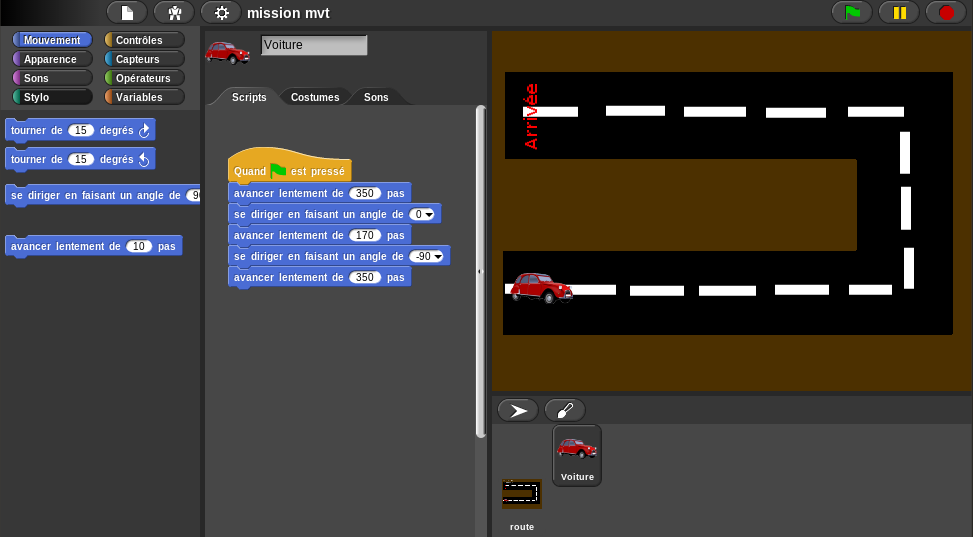
\includegraphics[width=\textwidth]{content/7-solution/1-missions/images/voiture}
    \caption{Mission de la voiture}
    \label{fig:mission-voiture}
  \end{center}
\end{figure}


\subsection{L'hélicoptère}
\label{mission-helicoptere}
Pour cette \gls{mission}, voir figure \ref{fig:mission-hélicoptère}, les élèves sont aux commandes d'un hélicoptère. Leur but est de faire le tour de la piste. La piste est un ellipsoïde bordé d'herbe. Cette forme ellipsoïde force les étudiants à utiliser des boucles et non un grand nombre de \glspl{bloc} créant une solution particulière. Si l'hélicoptère touche l'herbe, il explose. Sur le contour extérieur de la piste, une bande rouge et une bande bleue sont dessinées. Le but de cette \gls{mission} est de tourner dés qu'une de ces deux couleurs est touchée pour éviter l'explosion de l'hélicoptère. Comme pour la \gls{mission} précédente, à chaque lancement de \gls{script}, l'hélicoptère se repositionne à son point de départ.\\

Les concepts introduits par cette \gls{mission} sont :
\begin{itemize}
\item les boucles, particulièrement le \texttt{boucler infiniment} ;
\item la gestion des collisions grâce aux capteurs de couleurs ;
\item la division en sous-processus (un pour avancer, un pour la collision rouge et un pour la bleue).
\end{itemize}

\begin{figure}
  \begin{center}
    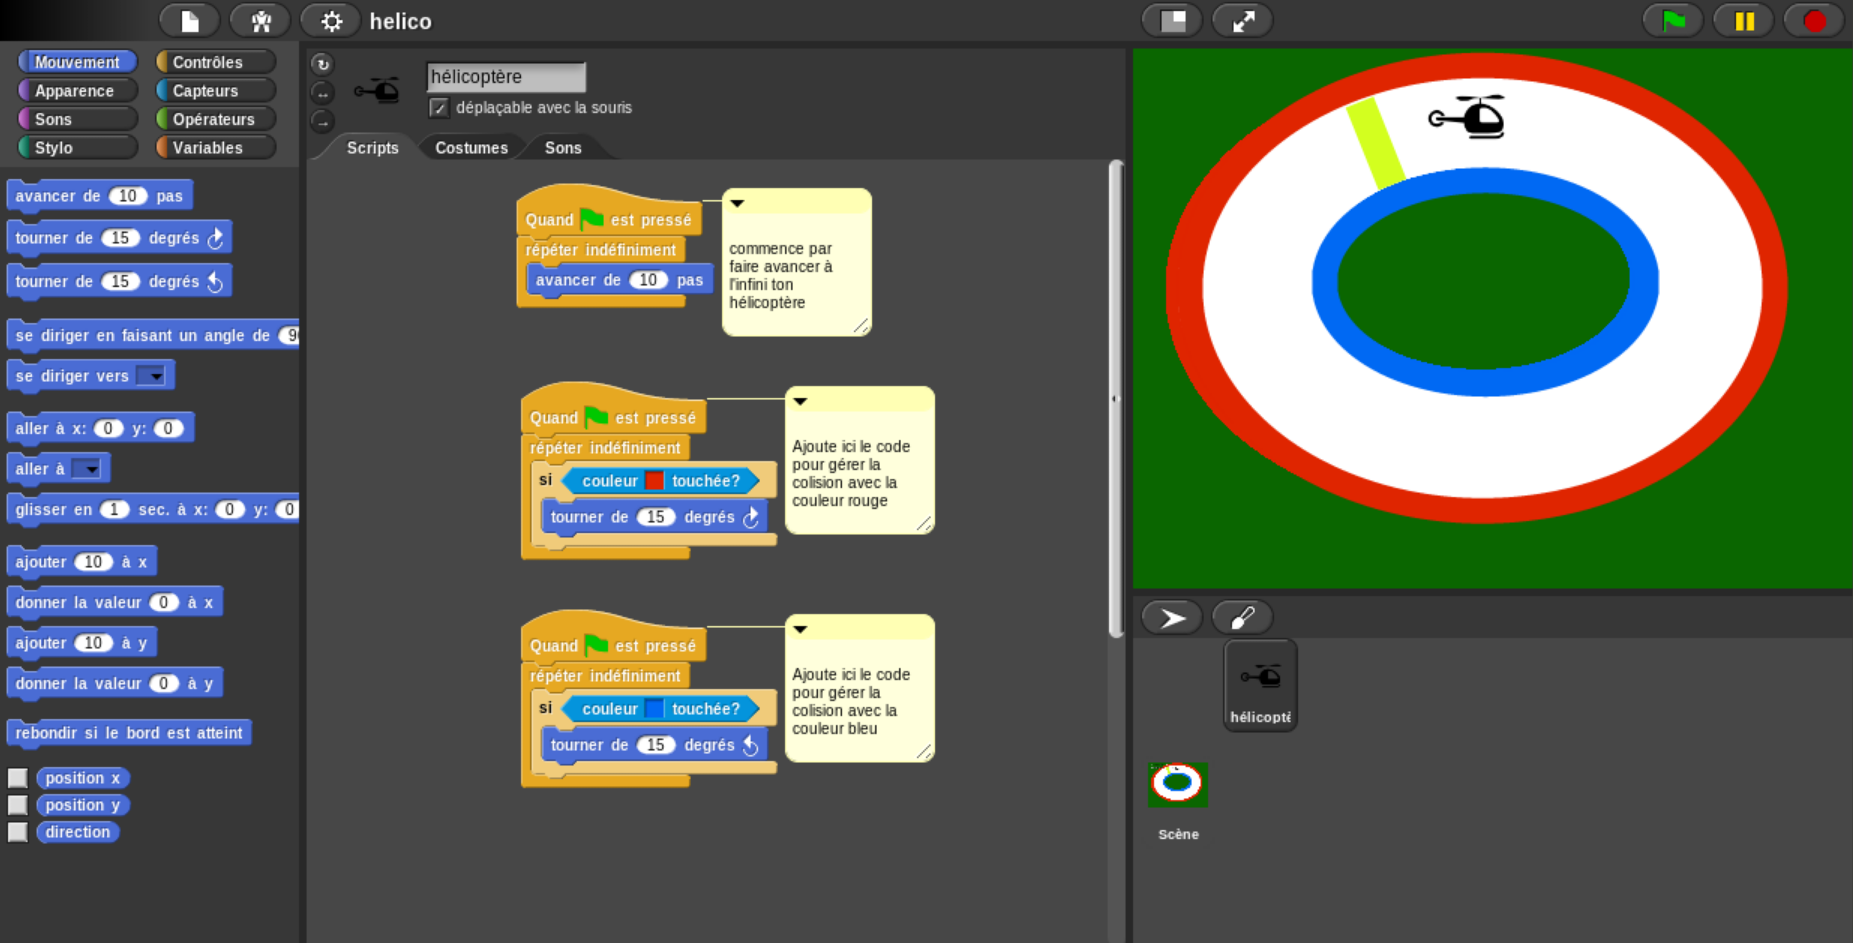
\includegraphics[width=\textwidth]{content/7-solution/1-missions/images/helicoptere}
    \caption{Mission de l'hélicoptère}
    \label{fig:mission-hélicoptère}
  \end{center}
\end{figure}

\subsection{Soyons courtois}
\label{mission-courtois}
Dans cette dernière \gls{mission} de préparation, voir figure \ref{fig:courtois}, les participants dirigent un personnage qui croise d'autres personnages. Ces derniers disent bonjour à chaque fois qu'ils croisent quelqu'un. Le but de la \gls{mission} est que le personnage de l'élève réponde.

Les concepts introduits par cette \gls{mission} sont :
\begin{itemize}
\item la gestion des collisions grâce au capteur sur leur personnage ;
\item la division en sous-processus (un pour chaque personne) ;
\item l'introduction à l'interactivité de l'interface, leur personnage est déplaçable à l'aide des flèches du clavier. ;
\item la gestion des dialogues et de l'affichage de textes.
\end{itemize}

\begin{figure}
  \begin{center}
    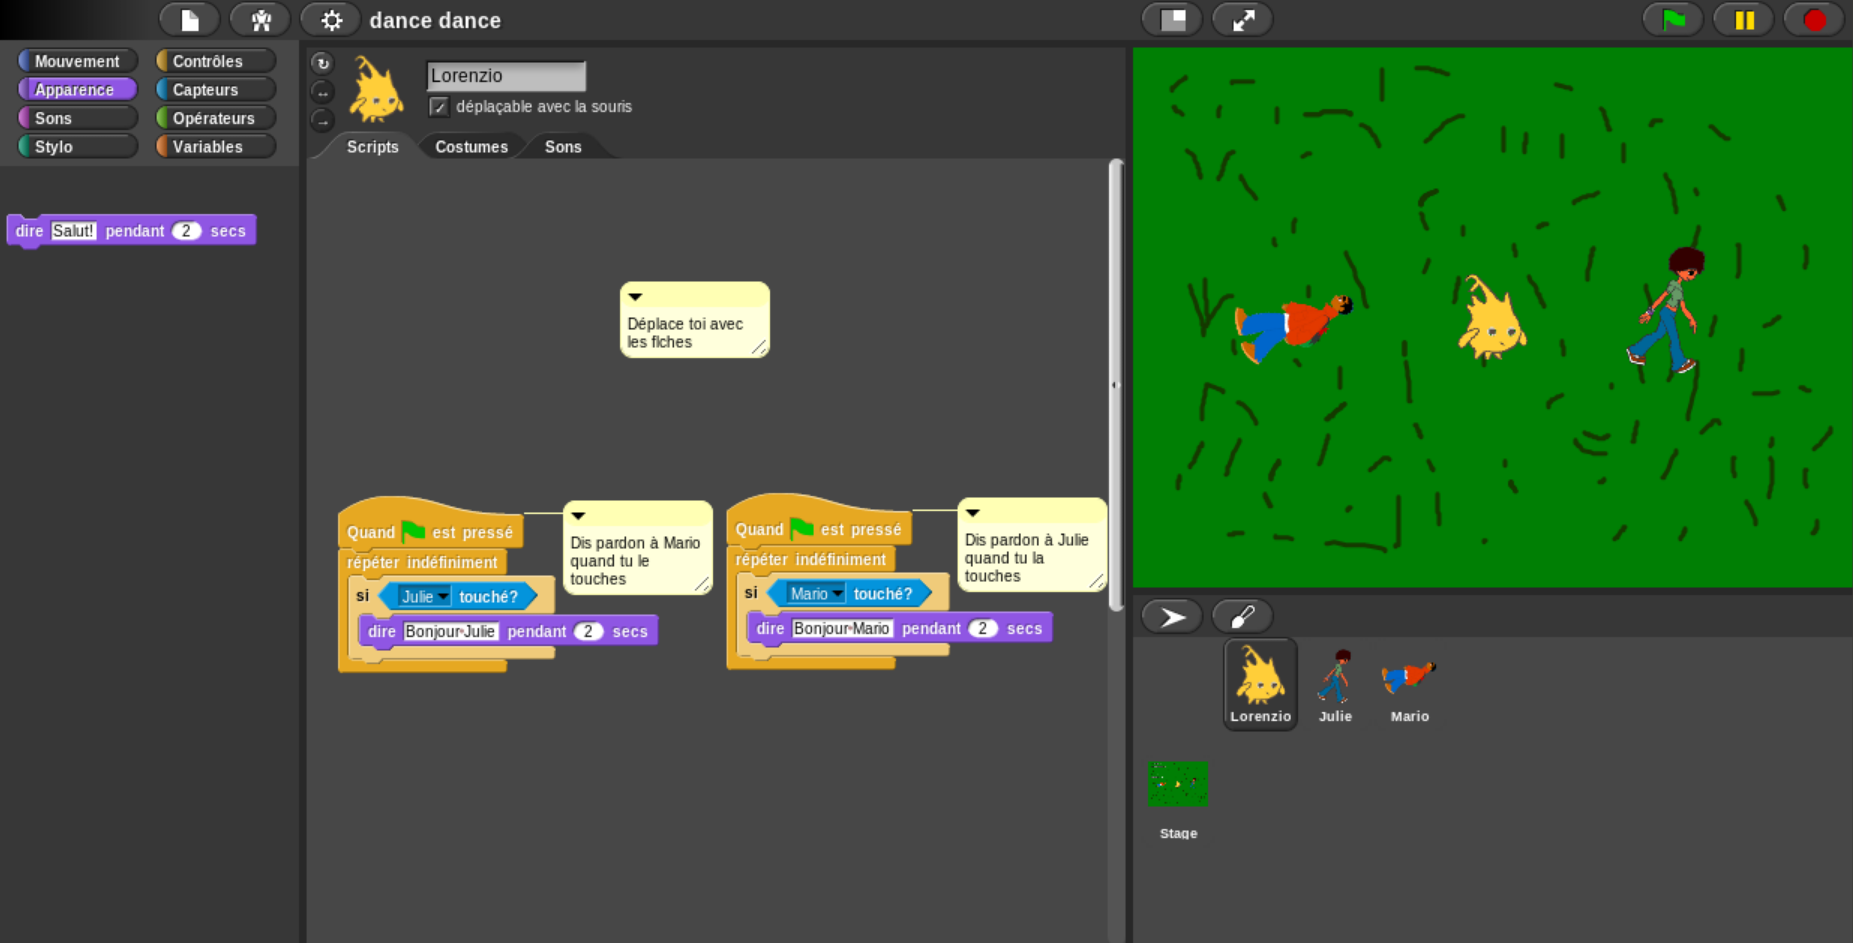
\includegraphics[width=\textwidth]{content/7-solution/1-missions/images/courtois}
    \caption{Mission de soyons courtois}
    \label{fig:courtois}
  \end{center}
\end{figure}

\subsection{Tu ne m'attraperas jamais}
\label{chien-chat}
Cette \gls{mission} est la dernière de la série et a pour but de mettre ensemble tous les concepts vus dans les \glspl{mission} de préparations. Dans cette \gls{mission}, les étudiants doivent faire en sorte d'avoir deux personnages et de pouvoir les déplacer séparément à l'aide des touches. Le chien doit courir après le chat. Sur base de propositions faites, les participants déterminent librement l'application exacte des effets de la poursuite. Par exemple, si le chat est touché par le chien, il crie.\\

Cette \gls{mission} reprend les concepts vus dans les \glspl{mission} de préparation auxquels elle ajoute :
\begin{itemize}
\item modification de l'interface de jeu ;
\item l'activation d'un \gls{script} sur un événement (déplacements) ;
\end{itemize}

En ce qui concerne les déplacements, ils sont déjà présents dans la \gls{mission} précédente, mais à l'état passif. Les étudiants ne font que l'utiliser. Dans cette \gls{mission}, ils doivent coder eux-mêmes le fait de pouvoir déplacer leur personnage à l'aide du clavier. Cette application approfondie du concept de déplacement fixe un concept important pour utiliser une interaction avec le clavier.

%analyse mission voiture, cela à permis de prendre en main les entrées des \glspl{bloc}. Au début, beaucoup prennent 3 \glspl{bloc} avancer de 10 pas pour faire 30 pas au lieu de changer la valeur du 10 en 30.

\section{Snap!}
\label{solution SNAP}
Ce travail part d'un environnent de programmation existant : \gls{snap}. Ce projet a pour but de fournir une interface et un environnement supportant la programmation par \glspl{bloc}. Cependant, ce projet ne s'inscrit pas dans le cadre d'un apprentissage scolaire ou guidé. Il a donc fallu l'adapter. Cette partie explique les différentes adaptations apportées au projet d'origine et pourquoi elles sont nécessaires pour remplir les objectifs.\\

Dans les adaptations opérées, sont retenus : une simplification de l'interface, une différenciation de rôle entre le professeur et le public cible, le masquage des scripts, une amélioration de la traduction en français et la sauvegarde sur les serveurs du projet courant.

\subsection{L'interface}
\label{interface}
Comme expliqué précédemment, \gls{snap} n'a pas une vocation didactique de groupe et a un public cible plus large. Il a des menus pour des fonctionnalités de gestion de l'ordonnanceur, des options d'affichage, des paramètres d'éditions, etc. Certaines de ces fonctionnalités sont trop complexes et/ou peuvent distraire inutilement le public visé par \gls{Rsnap}.

Un nettoyage en profondeur de l'interface de \gls{snap} a été opéré afin de laisser uniquement les menus utiles. Toutefois, il n'ont pas été effacés mais masqués afin qu'il puissent être utilisés par les professeurs, comme il est discuté dans les rôles \ref{role}.\\

Une autre adaptation de l'interface est l'ajout d'un menu pour les interactions avec la plateforme web. Ce menu contient des boutons tels que :
\begin{itemize}
  \item "sauvegarder sur le serveur", pour enregistrer le travail de l'étudiant sur la plateforme ;
  \item "description", pour permet de retrouver le résumé introductif de la mission ;
  \item "retour à la liste des missions", pour sauvegarder le travail puis renvoyer vers la page listant les missions sur le site web.
\end{itemize}

\subsection{Les rôles}
\label{role}
Afin de fournir une interface épurée pour les étudiants comme expliqués dans la section \ref{interface}, il est nécessaire d'enlever des parties non pertinentes de l'interface de \gls{snap}. Toutefois, ces options inutiles aux étudiants peuvent l'être pour les professeurs et également pour une mission en "mode ouvert". Il est donc utile d'avoir une interface modulaire suivant son utilisation. \\

Pour différencier les utilisations de l'interface, la notion de rôles a été ajoutée. Deux rôles sont définis : étudiant et professeur. Ainsi, quand un élèves ouvrent un projet, \gls{snap} est lancé avec le rôle étudiant, ce qui permet de ne pas afficher les options superflues. Quand un professeur souhaite modifier une mission ou en créer une nouvelle, \gls{Rsnap} lance \gls{snap} avec le rôle professeur ce qui donne accès aux fonctions avancées de \gls{snap}.\\

Ces rôles permettent également la gestion du masquage de script. Il est intéressant qu'un professeur puisse masquer des \glspl{bloc}, sans que les étudiants ne puissent les réafficher.

\subsection{Masquer les scripts}
Pour la création des missions, il a été nécessaire de cacher des \glspl{bloc} aux élèves. Par exemple, la partie de vérification du code de l'élève ou encore le code de l'environnement de la mission ne doivent pas leur apparaître.

Une possibilité de cacher des \glspl{bloc} existait déjà dans la zone des \glspl{bloc} sources (voir la figure \ref{fig:cacher}) de l'interface. Cette fonctionnalité est étendue pour pouvoir également cacher des \glspl{bloc} ou des scripts dans la partie d'édition (voir la figure \ref{fig:snap interface}).

Il a donc fallu ajouter cette information dans la sauvegarde du projet. Ceci a été réalisé grâce à la balise \texttt{hidden} dans le XML.\\


Cette fonctionnalité étant intéressante pour le projet original, elle a été proposée dans une \texttt{\gls{pull}}. Les responsables de \gls{snap} ont marqué leur intérêt pour cette fonctionnalité qui est toujours en cours d'étude.
\begin{figure}
  \begin{center}
    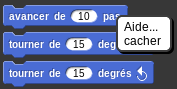
\includegraphics[scale=0.5]{content/7-solution/2-snap/images/cacher}
    \caption{Option pour cacher la définition d'un bloc}
    \label{fig:cacher}
  \end{center}
\end{figure}

\subsection{Traduction}
Ce travail se différencie des autres initiatives similaires introduites dans la section \ref{travail associe} par sont caractère francophone. L'application était déjà traduite partiellement en français mais une large majorité des traductions était incomplète, inexistante ou erronée. Il a donc fallu en améliorer la traduction. La traduction de l'application est différente pour la partie interface et la partie fournissant les aides.

Des aides étaient déjà disponibles en anglais. La possibilité de les avoir dans d'autres langues a été développée pour ce travail. De plus, des aides en français étaient déjà existantes dans le projet SCRATCH \cite{scratch-translation}. C'est donc elles qui ont été utilisées pour \gls{snap}.

L'ensemble de ces aménagements a été proposé au projet original. Il a été accepté et il sera intégré après quelques modifications du serveur utilisé par \gls{snap}.

\subsection{Sauvegarde sur le serveur}
Comme il est nécessaire d'interfacer l'environnement de programmation avec un site web, l'implémentation de certaines fonctionnalités d'import-export spécifiques à \gls{Rsnap} a été réalisée.

Il est nécessaire de disposer d'un fichier XML pour sauvegarder les missions sur le serveur. Les fonctions existantes ont été adaptées pour permettre d'avoir ce fichier et de pouvoir l'envoyer au serveur.

\section{Rsnap}
\graphicspath{{content/7-solution/3-rsnap/images/}}
Cette section traite de l'implémentation de la solution \gls{rsnap} ainsi que d'une présentation de son utilisation.

\subsection{Implémentation}
Comme expliqué en section \ref{rails}, \gls{rails} possède une architecture Model-Vue-Controleur. Cette section va présenter l'application en se basant sur ce modèle d'architecture. La première partie explique le modèle, ensuite les contrôleurs sont abordés. Enfin, les vues sont présentées.

\subsubsection{Modèles}
Les concepts utiles pour développer l'application sont ceux présentés par les différents modèles dans la figure \ref{fig:models}.

\begin{figure}
 \begin{center}
   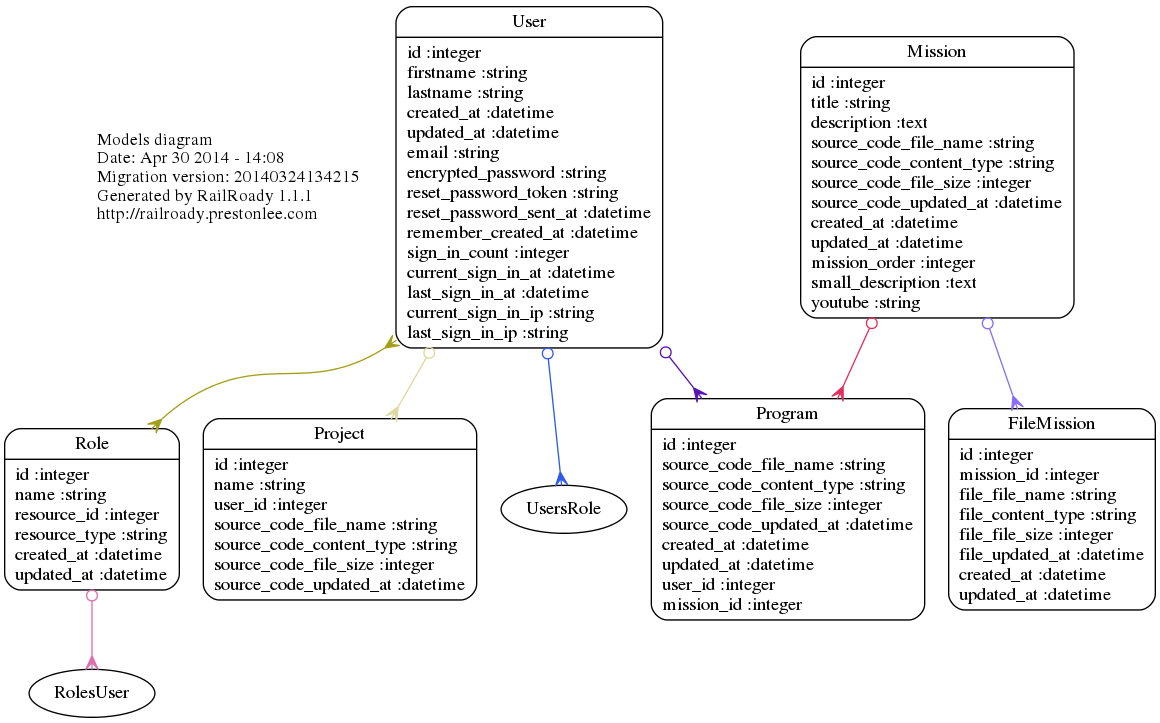
\includegraphics[width=\textwidth]{models_complete}
   \caption{Modèles de Rsnap}
   \label{fig:models}
 \end{center}
\end{figure}

\paragraph{\texttt{User}} Ce modèle contient les informations nécessaires pour identifier les utilisateurs (\texttt{firstname}, \texttt{email} \ldots) et pour les authentifier (\texttt{encrypted\_password}, \texttt{current\_sign\_in\_ip}, \ldots). Les utilisateurs peuvent posséder plusieurs \glspl{role}, programmes et projets.

\paragraph{\texttt{Role}} Les \glspl{role} permettent de donner des attributs aux utilisateurs. Ce modèle a été généré automatiquement par Rolify \ref{rolify}. Dans le cas de \gls{rsnap}, deux types d'utilisateurs ont été créés : \texttt{admin} et \texttt{teacher}. Ces deux \glspl{role} sont globaux et ne sont donc pas rattachés à une ressource spécifique.

Les \glspl{role} sont utiles en conjonction avec les autorités \ref{authority} pour donner des droits supplémentaires à ces types d'utilisateurs.

\paragraph{\texttt{Mission}} Les \glspl{mission} représentent tout ce qui est nécessaire pour avoir un exercice. Une \gls{mission} comporte donc un titre, une description avec des images et une vidéo pour expliquer à l'élève ce qu'il devra faire. De plus, elle comporte le code source initial de l'exercice. Généralement, celui-ci contient le squelette initial du programme pour l'élève et les tests pour vérifier le programme.

\paragraph{\texttt{FileMission}} Les fichiers liés à une \gls{mission} sont les différentes images qui composent la description.

\paragraph{\texttt{Program}} Les programmes contiennent la solution d'une \gls{mission}. Ils contiennent uniquement le code source de l'élève.

\paragraph{\texttt{Project}} Les projets sont identiques aux programmes, mais ne sont pas liés à une \gls{mission}. Ils contiennent donc le nom du projet en plus du code source.

\paragraph{Exemple} \texttt{Program} est un bon exemple de modèle \gls{rails} (code source \ref{lst:model-program}). Seules les fonctionnalités qu’Active Record \ref{active-record} ne sait pas déduire de lui-même sont présentes. Le modèle contient donc uniquement :
\begin{itemize}
  \item le nom des modèles avec qui il est associé et la cardinalité de la relation (\lstinline[language=Rails]{belongs_to} ligne 5-6) ;
  \item la validation de certains attributs pour qu'ils respectent certaines contraintes (\lstinline[language=Rails]{validates} ligne 13-15) ;
  \item des méthodes de classes pour simplifier les requêtes au modèle (\lstinline[language=Rails]{scope},  \lstinline[language=Rails]{self.*} ligne 17-23).
\end{itemize}

Comme c'est visible pour les \lstinline[language=Rails]{scope} à la ligne 17-19, Active Record permet de faire des requêtes SQL directement en Ruby.
\begin{figure}
\lstinputlisting[language=Rails, firstline=21, caption={Modèle \texttt{Program}}, label=lst:model-program]{content/7-solution/3-rsnap/listings/program.rb}
\end{figure}

\subsubsection{Contrôleurs}
Les contrôleurs donnent accès à différentes ressources. La figure \ref{fig:controllers} montre la liste des contrôleurs implémentés pour cette application. La majorité de ceux-ci se rapporte directement à un modèle spécifique. Il existe néanmoins certaines ressources différentes telles que :
\begin{itemize}
  \item les pages statiques (\texttt{HomeController}) ;
  \item l'ordonnancement des \glspl{mission} (\texttt{SortMissionsController}) ;
  \item la création d'un programme depuis une \gls{mission} (\texttt{InitializationMissionController}) ;
  \item les ressources utiles à l'affichage de \gls{snap} (\texttt{SnapAssetsController}).
\end{itemize}

\begin{figure}
 \begin{center}
   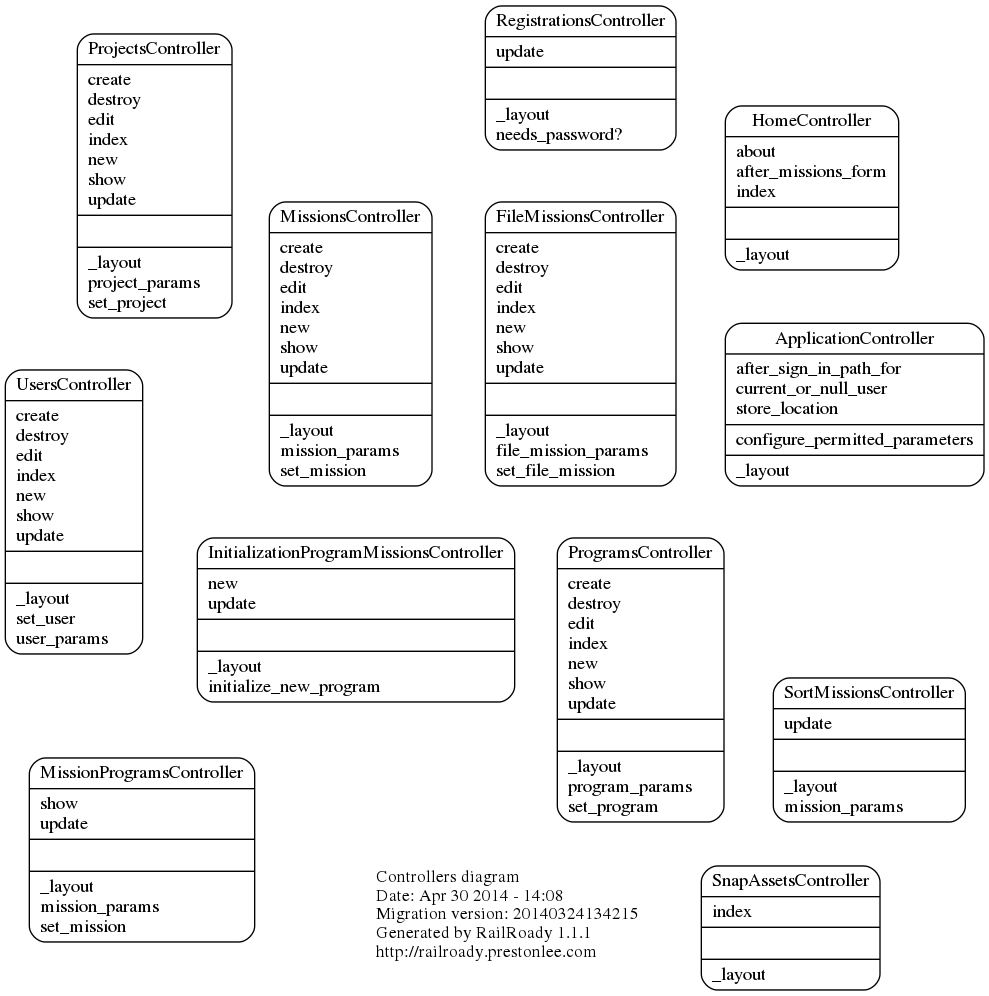
\includegraphics[width=\textwidth]{controllers_complete}
   \caption{Controlleurs de Rsnap}
   \label{fig:controllers}
 \end{center}
\end{figure}

Comme il est expliqué dans la section \ref{controleur}, les méthodes accessibles sont définies dans \texttt{routes.rb}. Les contrôleurs ont tous des ressources \gls{rest} excepté \texttt{HomeController}. Ceci est visible dans \texttt{routes.rb} ou en regardant les fonctions publiques disponibles dans les contrôleurs sur la figure \ref{fig:controllers}.

\paragraph{Exemple}
L'extrait du contrôleur \texttt{MissionsController} \ref{lst:controller-mission} montre l'usage classique d'un contrôleur.

\begin{figure}
\lstinputlisting[language=Rails, linerange={1-5,10-34,52-62}, caption={Extrait du controlleur \texttt{MissionsController}}, label=lst:controller-mission]{content/7-solution/3-rsnap/listings/missions_controller.rb} %TODO vérifier les ranges des lignes
\end{figure}

Grâce au méta-programmation, \lstinline[language=Rails]{authorize_actions_for Mission} permet de rajouter, sur toutes les méthodes \gls{rest}, des vérifications de ce que peut réaliser ou pas l'utilisateur courant. Ces vérifications sont injectées dans les autorités \ref{autority}. De plus, la méthode \lstinline[language=Rails]{before_filter} donne la possibilité de réaliser une action supplémentaire avant chaque appel de fonction. Dans cet exemple, il faut que l'utilisateur soit authentifié pour que l'application puisse ensuite vérifier ses droits. Ceci à l'exception des actions \texttt{show} et \texttt{index} qui peuvent être publiques.

Dans une méthode publique d'un contrôleur plusieurs actions sont à implémenter :
\begin{enumerate}
  \item traiter, si nécessaire, les paramètres fournis. Ceux-ci se trouvent dans \lstinline[language=Rails]{params} ;
  \item Assigner les variables d'instance dont la vue a besoin pour s'afficher correctement ;
  \item Exécuter le rendu de la page. Cette étape est facultative si la vue a le même nom que la méthode.
\end{enumerate}

\subsubsection{Vue}
\label{vues}
Les vues sont écrites en haml \ref{haml}.

L'exemple de code \ref{lst:vue-user-index} avec \ref{lst:vue-user-partial} montre comment la vue servant à lister tous les utilisateurs est représentée (figure \ref{fig:vue-users}).

\begin{figure}
\lstinputlisting[language=haml, caption={Vue \texttt{index} des utilisateurs}, label=lst:vue-user-index]{content/7-solution/3-rsnap/listings/index.html.haml}
\end{figure}

Le code source \ref{lst:vue-user-index} montre comment sont utilisées les variables d'instance créées par le contrôleur. Par exemple, la variable \texttt{@title} sert de titre 1.

\begin{figure}
\lstinputlisting[language=haml, caption={Vue d'une ligne \texttt{\_user} représentant un utilisateur}, label=lst:vue-user-partial]{content/7-solution/3-rsnap/listings/_user.html.haml}
\end{figure}
De plus, \gls{rails} permet de faire le rendu d'un autre fichier de manière élégante. La ligne 14 du code source \ref{lst:vue-user-index} exécute le rendu sur tous les éléments de la collection \texttt{users} grâce au fichier \ref{lst:vue-user-partial}

Les connaisseurs de Bootstrap \ref{bootstrap} auront reconnu l'usage intensif des classes de style qu'il propose. L'adaptativité de cet outil est visible sur la capture d'écran \ref{fig:vue-users} : le menu supérieur a été réduit, car la taille de l'écran était trop petite pour accueillir le menu en entier.

\begin{figure}
  \begin{center}
    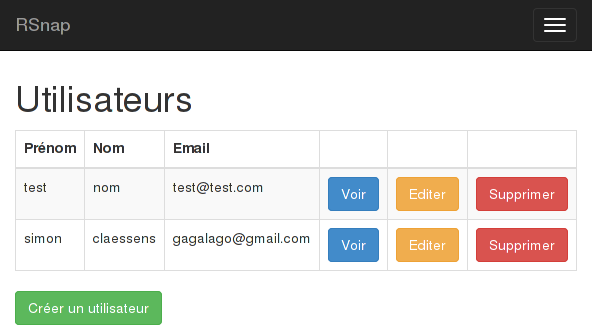
\includegraphics[width=.8\textwidth]{users}
    \caption{Affichage de la vue présentée par le code source \ref{lst:vue-user-index} et \ref{lst:vue-user-partial}}
    \label{fig:vue-users}
  \end{center}
\end{figure}

\subsection{Utilisation}
Pour utiliser la plateforme, il faut d'abord s'enregistrer. Ensuite, suivant le profil, différentes actions sont possibles. L'utilisateur normal peut uniquement résoudre les \glspl{mission} dans l'ordre proposé par les professeurs. Les professeurs peuvent aussi créer des \glspl{mission}. Cette section présente l'utilisation de la plateforme.
%TODO screenshot en annexe

\paragraph{Professeur}
Si un professaur veut lui-même réaliser un cours de programmation, il doit pouvoir faire les actions suivantes.

\subparagraph{Créer des missions} Pour créer une nouvelle \gls{mission} (figure \ref{fig:mission-create}), le professeur se rend sur la page qui liste toutes les \glspl{mission}. Ensuite, il clique sur le bouton en bas de page "Nouvelle mission". Sur la page suivante, il donne les informations sur la \gls{mission} : titre, description, explication de la mission, vidéo d'explication \ldots Il lui reste à créer la mission proprement dite. Lorsque le professeur clique sur le bouton "Créer une \gls{mission}", il est redirigé vers l'interface de \gls{snap}. Il peut alors créer tout ce qui est nécessaire à la réalisation et au test de la mission. Avant de sauver, il ne doit pas oublier de cacher les \glspl{bloc} et les \glspl{script} qui ne doivent pas être visibles par les élèves.
\begin{figure}
  \begin{center}
    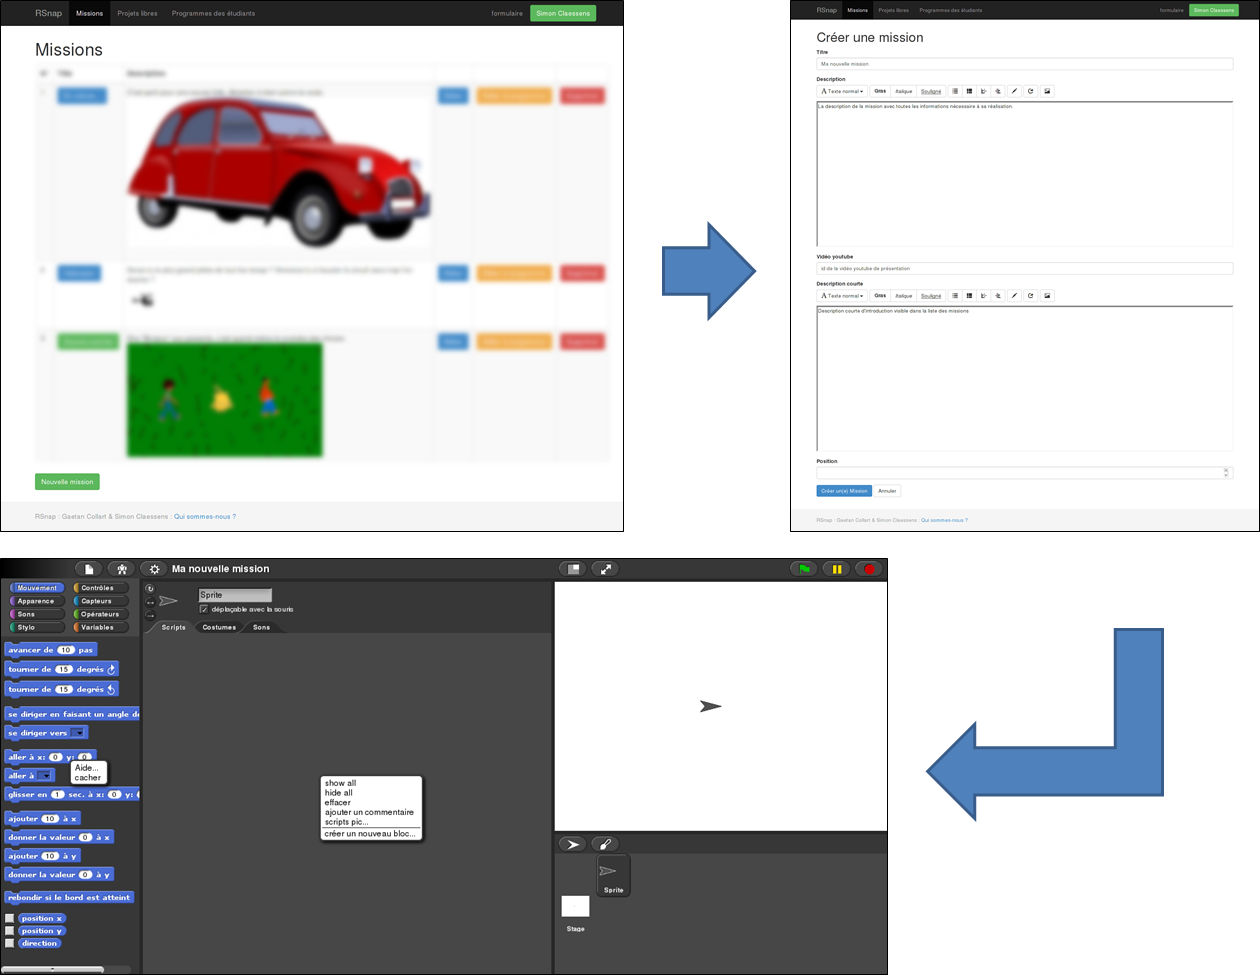
\includegraphics[width=.9\textwidth]{mission-create}
    \caption{Création d'une mission}
    \label{fig:mission-create}
  \end{center}
\end{figure}

\subparagraph{Ordonner les missions} Pour ordonner les \glspl{mission} (figure \ref{fig:mission-order}) dans un ordre pédagogique, il suffit de les glisser dans la liste.
\begin{figure}
  \begin{center}
    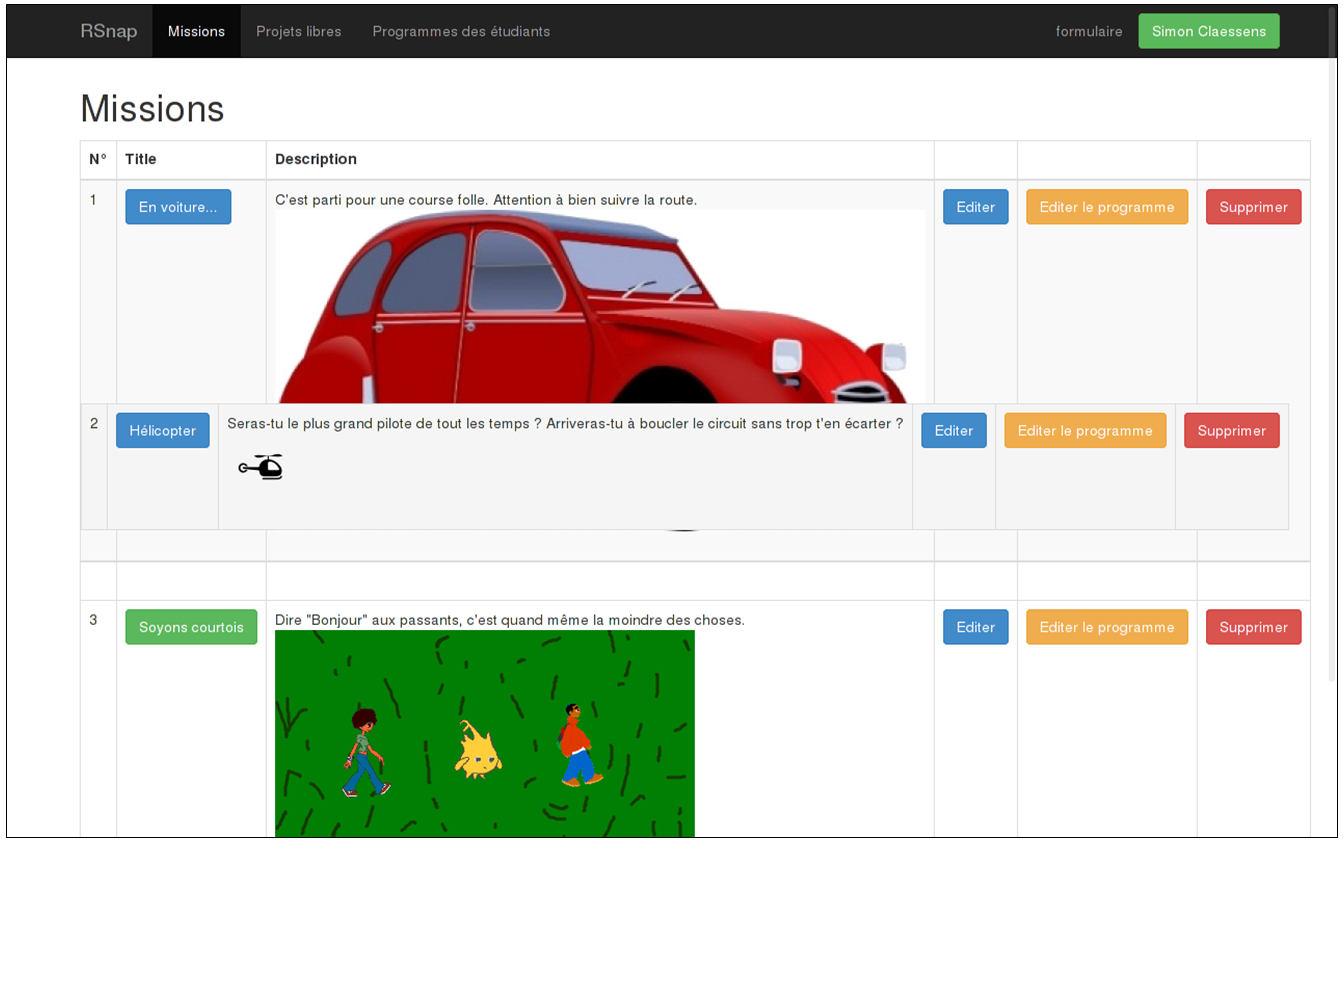
\includegraphics[width=.9\textwidth]{mission-order}
    \caption{Ordonner les missions}
    \label{fig:mission-order}
  \end{center}
\end{figure}

\subparagraph{Corriger les soumissions des élèves} Pour corriger les soumissions de ses élèves (figure \ref{fig:program-correction}), le professeur se rend sur la page des programmes. Il y sélectionne le programme qu'il désire corriger et qui s'ouvre dans l'interface \gls{snap}. Le professeur peut alors rajouter des commentaires.
\begin{figure}
  \begin{center}
    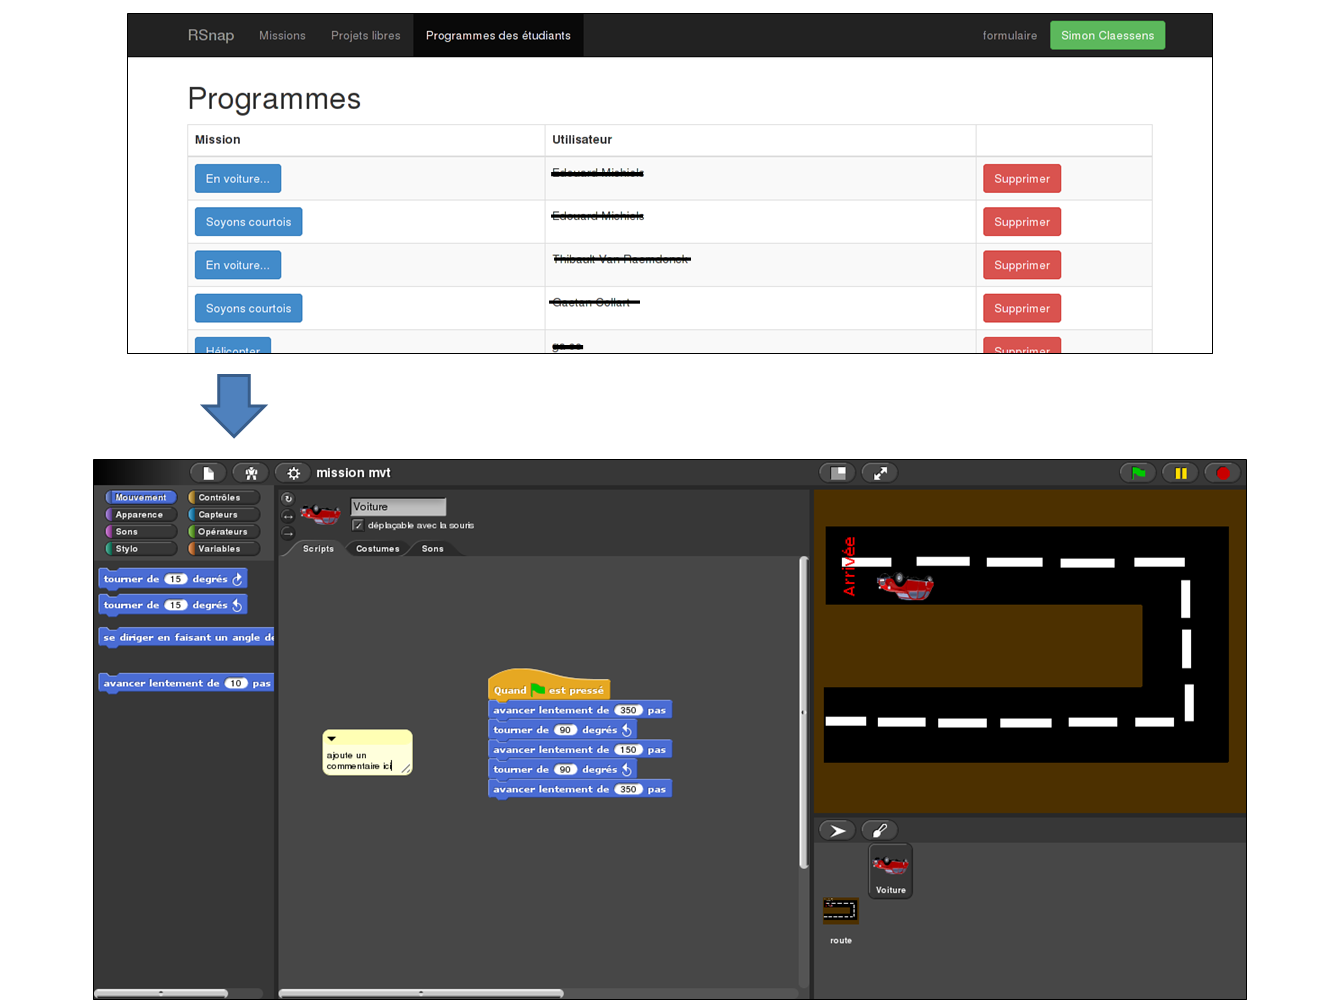
\includegraphics[width=.9\textwidth]{program-correction}
    \caption{Correction d'un programme}
    \label{fig:program-correction}
  \end{center}
\end{figure}

\paragraph{Étudiant}
Un élève doit pouvoir réaliser les opérations suivantes.

\subparagraph{Réaliser une mission} L'élève réalise une \gls{mission} (figure \ref{fig:program-creation}) en cliquant sur le nom de la \gls{mission}.

Deux possibilités s'offrent à lui. Soit le bouton est bleu, ce qui signifie que la \gls{mission} a déjà été commencée. L'élève la reprend là où elle s'était arrêtée. Soit, le bouton est vert et dans ce cas, une nouvelle \gls{mission} commence.

Dans les deux cas, l'élève se retrouve sur l'interface de \gls{snap}.
\begin{figure}
  \begin{center}
    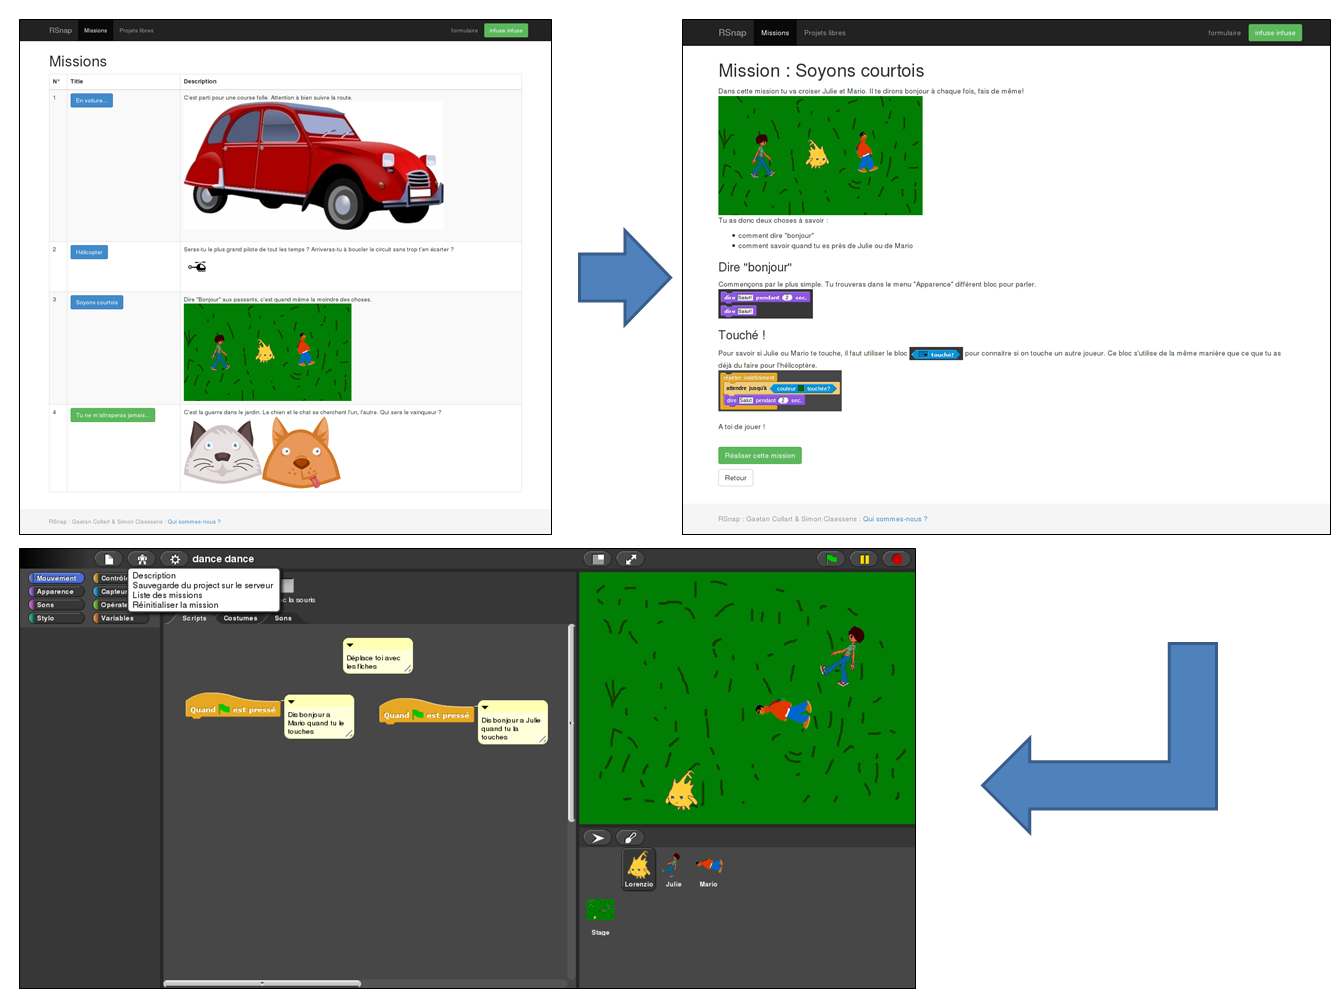
\includegraphics[width=.9\textwidth]{program-creation}
    \caption{Réalisation d'une mission}
    \label{fig:program-creation}
  \end{center}
\end{figure}

\subparagraph{Réaliser un projet libre} Si l'élève a envie de créer quelque chose (figure \ref{fig:project}), il va dans le menu "projet libre". Il utilise \gls{snap} à son plein potentiel et laisse libre cours à son imagination pour créer le programme de ses rêves.
\begin{figure}
  \begin{center}
    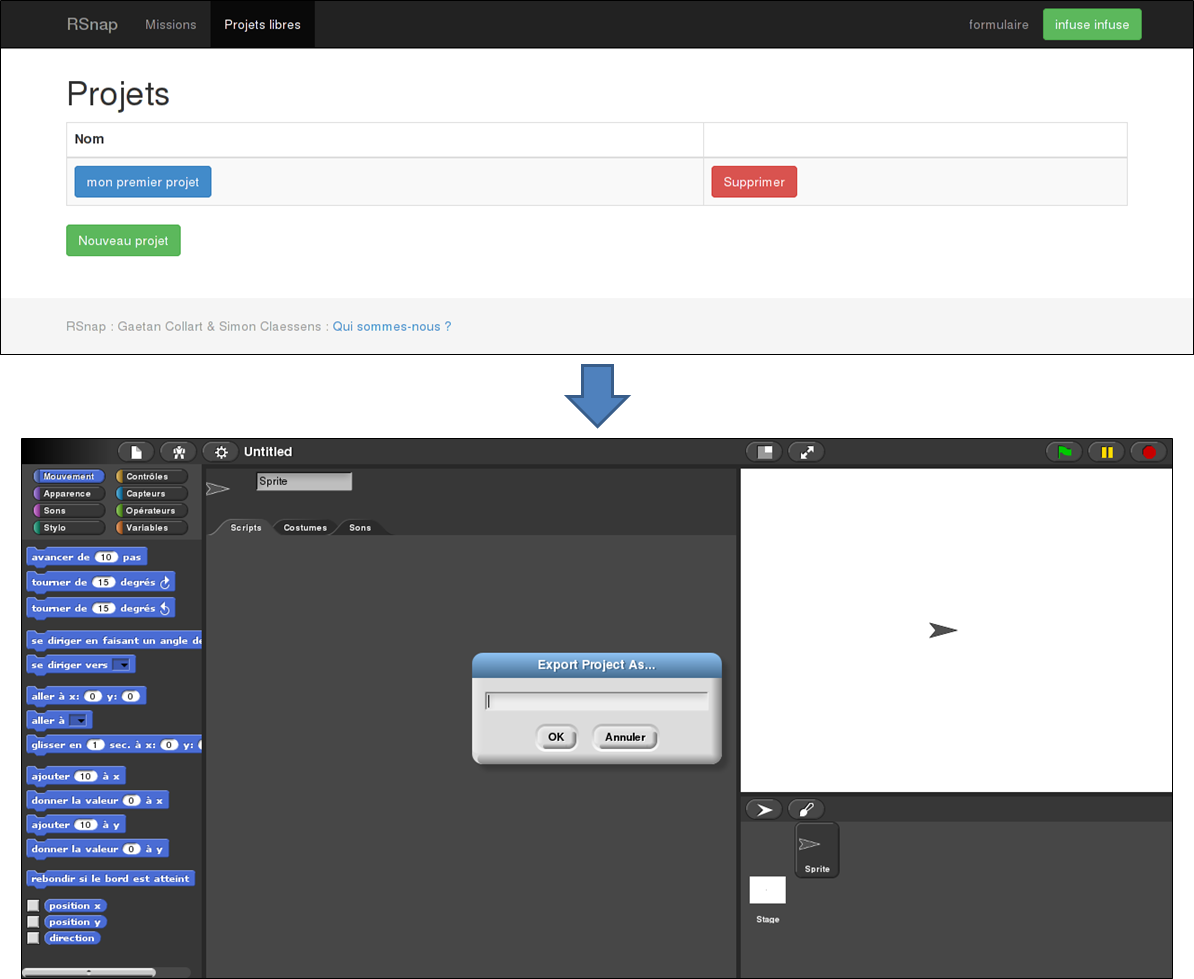
\includegraphics[width=.9\textwidth]{project}
    \caption{Réalisation d'un projet libre}
    \label{fig:project}
  \end{center}
\end{figure}


\chapter{Validation}
Ce chapitre présente les techniques de validation de la plateforme Rsnap. La validation du code est abordée dans un premier temps. Ensuite, les expériences sur des populations d'étudiants et leurs analyses sont développées.

\section{Implémentation}
Dans cette section, les outils de validation du code de Rsnap sont présentés. Deux outils principaux ont été utilisés pour avoir un logiciel le mieux écrit possible \ref{rails-tests} : les tests unitaires et les métriques.

\subsection{Tests unitaires}
Les tests unitaires servent à vérifier que le code fonctionne correctement. L'implémentation des tests s'est déroulée en parallèle à la création de l'application. Deux principaux types de tests ont été réalisés, ceux sur les contrôleurs et ceux au niveau de l'utilisateur. Avant de les aborder, un courte section présente les programmes utilisés pour les tests.

\subsubsection{Outils pour les tests}
Un des programmes utilisés pour les tests est Travis-CI (\ref{travis}). Ce programme est relié à Github pour que tous les tests soient exécutés à chaque commit sur le dépôt. De plus, lors d'une "pull request", les tests sont également effectués pour savoir si l'acceptation de la branche introduira des bogues.

Une des métriques générées par les tests est la couverture du code. Cette information est fournie par Coveralls\cite{coveralls} qui est liée à Travis-CI pour l'acquisition des données. Cette métrique est utile pour connaître la fraction du code couvert par les tests. Elle ne donne par contre pas d'information sur le type de code testé. Il faut donc être attentif à ce que les tests couvrent effectivement les parties critiques.

Enfin, lors des tests, il est nécessaire d'avoir des données pour peupler les modèles. Ceci s'effectue grâce au gem FactoryGirls \cite{factorygirls} qui propose un langage dédié pour écrire rapidement des fabriques. Ces dernières vont générer ces données de test pour peupler les modèles.

\subsubsection{Tests au niveau des contrôleurs}
Un premier type de tests est réalisé grâce à RSpec \cite{rspec}. Ces tests ont pour vocation de vérifier l'accès aux différentes routes \ref{rails-routes} : les droits des utilisateurs et le type de retour des contrôleurs.

Un exemple de test est visible sur dans le code source \ref{lst:rspec}. La partie \texttt{setup} utilise la fabrique spécifique pour créer une mission à chaque test. Deux tests sont ensuite réalisé qui vérifie que seul un utilisateur authentifié peut réaliser une mission.

\begin{figure}
\lstinputlisting[language=Ruby, caption={Test de l'accès au programme associé \`a une mission}, label=lst:rspec]{content/8-validation/validation/program_mission_initializations_controller_test.rb}
\end{figure}

\subsubsection{Tests au niveau de l'utilisateur}
Un deuxième type de tests est réalisé grâce à Cucumber \ref{cucumber}. Ces tests s'effectuent à partir du point de vue de l'utilisateur. Ils assurent le bon fonctionnement des fonctionnalités demandées par l'utilisateur ainsi que des ressources qui en dépendent. Ces tests sont donc de haut niveau, car ce n'est que via les interactions faites sur l'interface que des erreurs internes à l'application peuvent être trouvées.

\begin{figure}
\lstinputlisting[language=Gherkin, caption={Tests de l'accès aux missions}, label=lst:cucumber-mission]{content/8-validation/validation/mission_access.feature}
\end{figure}

\begin{figure}
\lstinputlisting[language=Ruby, linerange={1-15}, caption={Extrait de l'implémentation des tests de l'accès aux missions}, label=lst:cucumber-implementation-mission]{content/8-validation/validation/mission_steps.rb}
\end{figure}

Gerkin est utilisé pour écrire les scénarii en langage naturel. 
Le code source \ref{lst:cucumber-mission} montre différents scénarii décrivant l'accès aux missions. Le haut niveau de Gherkin est visible dans cet exemple. En effet, toute personne anglophone peut comprendre ce que testent les différents scénarii. 

L'extrait de code \ref{lst:cucumber-implementation-mission}, montre comment sont implémentés les scénarii précédents. La façon dont est piloté un navigateur pour réaliser les tests est aussi visible via les méthodes : \texttt{click\_on}, \texttt{current\_path}, \texttt{visit}\ldots

\subsection{Utilisation de metriques}
Un autre style d'outils donne des informations sur le projet via son code source. Deux services ont principalement été utilisés.

\subsubsection{Gemnasium}
Gemnasium \ref{gemnasium} permet d'avoir un service de veille qui vérifie si les dépendances de l'application sont bien à jour et qu'elles ne présentent pas de risque de sécurité.

\subsubsection{rails\_best\_practice}
rails\_best\_practice \ref{rbp} fournit quant à lui une information plus complexe à traiter. En effet, il renseigne les endroits dans le code source qui ne respecteraient pas le "rails way" et en fournit des exemples de réécriture. Cet outil est donc principalement utile en début de projet quand les auteurs ne connaissent pas encore bien quelles sont les bonnes pratiques.

\section{Expériences}
Cette section aborde les expériences réalisées pour ce travail. celles-ci commencent par un après-midi chez KidsCode. Vient ensuite le "Printemps des Sciences" pendant lequel environ 80 élèves ont testé l'application. Enfin, une analyse des expériences à travers des formulaires remplis par les élèves et les professeurs est approchée.

\subsection{KidsCode}
\label{kidscode}
La première expérience s'est déroulée chez KidsCode. Cette organisation a été présentée dans la section \ref{init-kidscode}. C'est une petite initiative locale qui apprend la programmation à 10 enfants âgés de 10 à 14 ans.

\subsubsection{Contexte}
\label{context-kidscode}
Il est important de définir le contexte et la publique de l'expérience qui en influencent considérable son analyse.

Lors de cette expérience, le public était composé de 10 enfants de 10 à 14 ans ayant déjà fait une demi-année de programmation dans le cadre du projet KidsCode. Le niveau de ces enfants n'est donc pas à négliger. Ils sont habitués à exécuter un programme et maîtrisent les principaux concepts de la programmation.

\subsubsection{Buts}
Le but poursuivi dans cette expérience est de valider l'utilisabilité de la plateforme et également le niveau de difficulté des missions proposées. 

Un autre but était de familiariser les expérimentateurs avec des utilisateurs en petit groupe, en vue de préparer la seconde expérience.
Même si ce dernier point pourrait sembler être moins justifié dans le cadre d'un mémoire sur l'informatique, l'aspect pédagogique rentre en ligne de compte dans le cadre de l'utilisation de l'application. Certains paramètres ont pu être identifiés et réfléchis pour leurs implications dans l'expérience ultérieure.
%Pour limiter le plus possible les biais dus à un manque de pédagogie ou d'expérience dans la gestion d'un groupe d'enfant, il était important de pouvoir avoir cette première expérience.

\subsubsection{Déroulement}
L'expérience s'est déroulée pendant un peu plus d'une heure. A la suite des activités habituelles de KidsCode, la dernière heure y était consacrée. 

Le début de l'expérience a été marqué par une perte d'attention et la dissipation des enfants. Une fois le groupe repris en main, les jeunes ont directement montré beaucoup d'intérêts, aussi bien pour l'interface qu'ils découvraient, que pour la compétition intergroupes qui s'est rapidement mis en place.

Comme expliqué dans la partie précédente \ref{context-kidscode}, le public avait déjà de bonnes notions de programmation par rapport au public visé par ce mémoire. Les premières missions ont donc été rapidement réalisées. Les principaux points de ralentissement étaient des problèmes de lecture des consignes. En effet, les auteurs n'avaient prévu que des consignes écrites. Or, les jeunes ne prenaient pas le temps de les lire et ne savaient donc pas quoi faire. Il semble que ce soit l'impatience des jeunes à mener les missions plus que leur niveau de lecture qui détermine leur comportement.

La compétition que les jeunes ont mise en place dès le début a eu un effet bénéfique pour leur évolution car elle leur donnait la motivation de réaliser les défis proposés. Ceci était fort visible à chaque passage de mission. Chaque fois qu'un groupe finissait sa mission, il était important pour lui de le signaler aux autres. Cela lui donnait une satisfaction qui le poussait à réaliser la mission suivante. 

Dans les délais impartis, alors que tous sont arrivés à la mission finale du chien et du chat \ref{chien-chat}, personne n'a réussi à la finir. 

Quand a sonné la fin de l'expérience, beaucoup de jeunes nous ont demandé comment faire pour montrer à leur famille ce qu'ils avaient réalisé et comment faire pour continuer la mission finale.

\subsubsection{Analyse}
\label{analyse-kidscode}
Dans l'ensemble, l'expérience s'est très bien déroulée et les participants ont beaucoup apprécié.

Cependant pour tenir compte de certains paramètres, des améliorations ont été apportées à l'application. Ces modifications sont abordées dans la suite de cette partie.

\paragraph{Changement dans les missions}
La mission \texttt{répète et répépète} a été retirée car elle s'est avérée peu accrocheuse pour les enfants et peu intéressante par rapport aux concepts introduits. Un personnage devait répéter ce que disait un autre. Pendant cette mission, beaucoup d'enfants se sont dispersés parce qu'ils s'embêtaient et que ce n'était pas assez concret. Cette mission avait pour but de faire découvrir les fonctions d'affichage de textes. 

Elle a été remplacée par \texttt{Soyons courtois} décrit en section \ref{mission-courtois}. Cette nouvelle mission est beaucoup plus dynamique que la précédente, car elle permet à l'étudiant de se déplacer et d'utiliseer les capteurs de collisions introduits dans la mission précédente.

\paragraph{Ajout d'un bouton "réinitialiser la mission"}
Lors de l'expérience, un groupe d'enfants a réussi à corrompre l'environnement de la mission suite à une série obscure d'opérations. Pour palier à ce genre de risque, un bouton "réinitialiser la mission" a été rajouté dans l'interface de Snap!. Il permet de réinitialiser la mission courante.

\paragraph{Ajout de vidéo d'introduction}
Comme observé dans cette expérience, les jeunes ont tendance à ne pas lire les textes explicatifs des missions. Il peut en résulter un manque de productivité. Une vidéo d'introduction a donc été rajoutée au début de chaque mission (figure \ref{fig:program-creation}). Cette vidéo explique le but de la mission et donne les instructions. En cas d'oubli, un résumé écrit est toujours présent.

\subsection{Printemps des Sciences}
Cette expérience s'est déroulée dans le cadre de la semaine Scienceinfuse. Des écoles du fondamental et du secondaire viennent participer à des animations dans les universités. L'expérience s'est déroulée avec quatre groupes d'enfants. Ces activités duraient une heure trente y compris les temps d'installation et de prise en charge. Les élèves étaient en programmation par paire \ref{paire} et donc à deux devant un ordinateur.

\subsubsection{Contexte}
Lors de cette expérience, 74 étudiants âgés de 11 à 13 ans étaient répartis en 4 classes, deux de sixième primaire et deux de première humanité.

L'origine des jeunes est également variée. Il y a eu des classes de Chimay, de Bousval et d'Ottignies, ce qui semble être un échantillon suffisamment représentatif.

\subsubsection{Buts}
Le but principal de cette expérience était de confronter l'application à son usage réel dans des classes d'étudiants. Il fallait pouvoir observer comment elle se déroule en réalité et en ressortir une analyse des besoins spécifiques de l'application.

Un autre but poursuivi était l'évaluation de l'âge idéal et du niveau de difficulté des missions pour des néophytes. En effet, lors de l'expérience précédente, le public était volontaire et avait déjà des connaissances en programmation. De par ce fait, le niveau des missions devait être afiné sur le public visé.

Les auteurs désiraient aussi observer les réactions et l'intérêt des étudiants pour la solution proposée.

Un dernier but était évidemment de récolter l'avis des étudiants. 

\subsubsection{Déroulement}
Le déroulement de cette expérience se divise en deux parties. La première présente le déroulement de l'activité commune aux écoles participantes. Ensuite vient une explication particulière à chaque écoles pour en détailler leurs spécificités.
\paragraph{Déroulement général des activités}
Lors de la mise en place de l'activité, une petite démonstration de l'interface a été présentée pour familiariser les étudiants à Snap!. 

Suite à cela, ils ont été invités à créer un compte par groupe de deux (par ordinateur).

Une fois la première vidéo passée, les élèves ont entamé la première mission.\\

La première mission était celle de la voiture, décrite à la section \ref{mission-voiture}. Les étudiants devaient y aborder un concept difficile, à savoir la structuration mentale de leur script. En effet, la voiture revenait à son point de départ à chaque lancement du script. Finalement, après quelques essais et erreurs, ils ont tous réussi cette mission.\\

Une fois la première mission finie, les auteurs ont du rappeler aux étudiants comment la sauver et comment revenir à la liste des missions. Ensuite, les élèves retrouvaient seuls comment continuer. 

Une question récurrente des étudiants était de savoir si leur mission avait bien été enregistrée sur le serveur.\\

À la fin de l'expérience, tous les participants ont reçu un diplôme avec l'adresse web de l'application, afin qu'ils sachent continuer leur programme chez eux.

\paragraph{École Sainte-Marie} 
La première classe à avoir testé l'application est une sixième primaire de l'école Sainte-Marie de Bousval. Le groupe était composé d'une petite vingtaine d'élèves.

L'activité s'est déroulée avec une petite contrariété informatique. En effet, l'interpréteur JavaScript des machines mises à disposition était très lent. Ceci n'a pas compromis le déroulement de l'activité, mais fut, à quelques moments, une source de frustrations pour certains élèves très enthousiastes.

À la fin du temps imparti, tous les élèves avaient atteint la dernière mission, décrit en section \ref{chien-chat}. Ils n'ont généralement pas fini l'étape de déplacement du personnage, mais étaient bien avancés en ce sens.

\paragraph{L'athénée royal Paule Delvaux}
Cette école est venue avec une classe de sixième primaire également. Pour cette expérience, le problème de réactivité de l'interface a été corrigé.

Par rapport a l'école de Bousval, les élèves semblaient avoir moins de facilité à comprendre et moins autonomes.
Cependant, ils sont arrivés à peu près aux mêmes résultats que ceux de Bousval.

L'enthousiasme des jeunes était également au rendez-vous et ils se sont bien amusés.

\paragraph{Collège saint Joseph}
Les deux dernières classes à participer à l'expérience étaient du collège saint Joseph de Chimay accompagnées par leur professeur de mathématique qui semblent induire auprès de leurs élèves un intérêt pour la logique, entre autres de programmation.

Comme ces deux classes avaient un niveau de première humanité, les enfants étaient plus autonomes. L'expérience s'est déroulée comme pour les primaires. La première mission était la plus laborieuse, mais une fois celle-ci passée, le reste a été plus aisé. Ces enfants étant plus grands, il a semblé aux auteurs qu'ils présentaient une capacité d'apprentissage plus élevée. En effet, ils ont été beaucoup plus rapides pour réaliser les missions. Ceci leur a permis d'avancer davantage dans la dernière mission. Certains groupes ont même réaliser un programme fonctionnel pour cette dernière mission: il ne manquait que le score à implémenter.\\

Dans ces classes une différence de niveau au sein des groupe a été observé. En effet certains duos étaient très autonome alors que d'autre se rapprochaient plus des groupes de l'enseignement fondamental.

\subsubsection{Analyse}
\label{analyse-scienceinfuse}
Tout en tenant compte des remarques précédentes, l'ensemble de ces expériences s'est globalement bien déroulée. Les objectifs ont été approchés. Le niveau des missions correspondait à ce qui était souhaité. La plupart des enfants a très vite et bien pris en main l'interface de Snap!. Les modifications apportées par la première expérience ont montré toutes leurs utilités. En autre, le bouton "réinitialisation" s'est avéré facile à utiliser. La mission \texttt{Soyons courtois}, voir section \ref{mission-courtois}, a été appréciée des enfants et a remplis pleinement son rôle.\\

Une crainte était que grâce au lecteur \texttt{YouTube}, ils regardent d'autres vidéos, mais il n'en fût rien et leur curiosité était assez forte pour les garder dans l'application.

Ces expériences ont mis en évidence d'autres améliorations possibles: 
\begin{itemize}
  \item ajouter un message d'information sur la sauvegarde des projets ;
  \item diminuer le taux de rafraîchissement de la fenêtre ;
  \item diviser la mission hélicoptère en deux missions séparées: la boucle "répéter indéfiniment" et la condition "si".
\end{itemize}

Par des expériences ludiques menées en une heure, les enfants ont appris des concepts basiques de la programmation. Les auteurs se sont rendu compte que beaucoup d'enfants n'avaient pas vu le temps passé.

\subsection{Analyse des formulaires}
\label{analyse-exp}
Un formulaire a été complèté par chaque enfants et chaque professeurs à la fin de l'activité. Dans cette partie, les formulaires sont analysés. Les données complètes, les graphiques et les commentaires sont disponibles en annexe \ref{annex-data-form}.

\paragraph{Niveau des enfants en informatique}
Une des questions du formulaire portait sur la connaissance de l'informatique et de la programmation. Les schémas montrent comment les enfants auto-évaluent leurs compétences en informatique et en programmation avant de faire l'expérience \ref{fig:niveau-avant} et après l'expérience \ref{fig:niveau-apres}.
\begin{figure}
  \begin{center}
    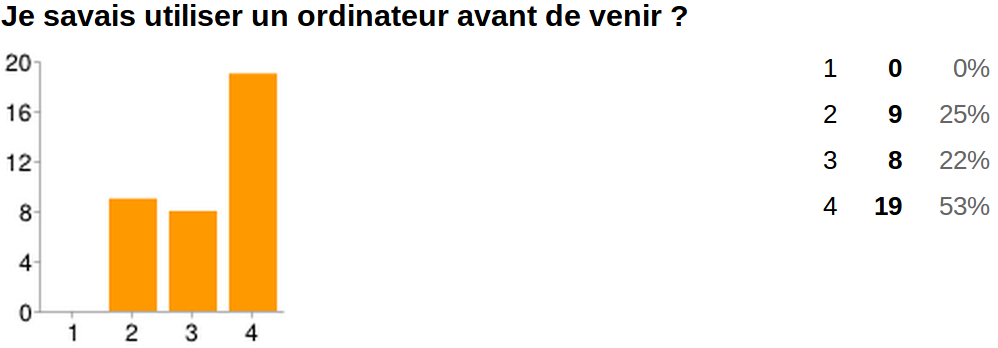
\includegraphics[width=.7\textwidth]{content/8-validation/images/avant}
    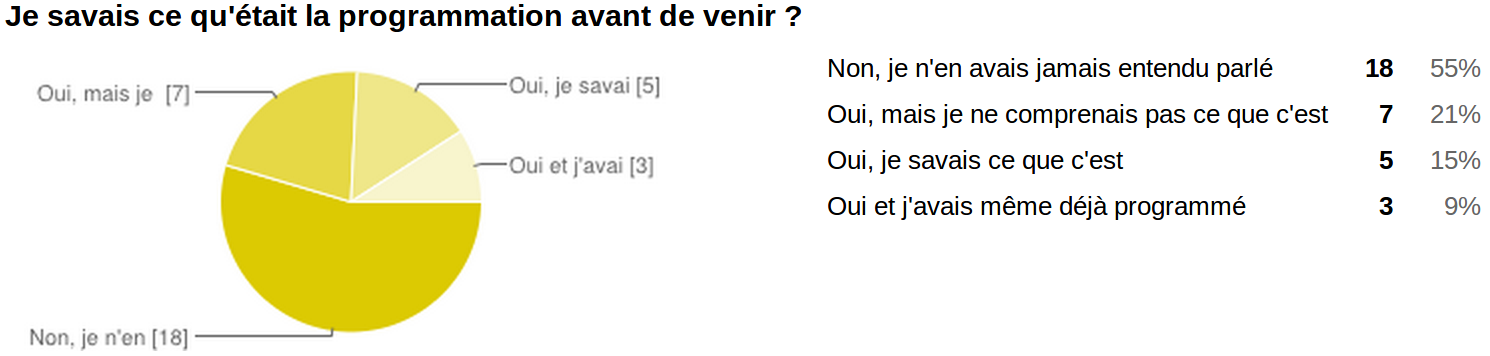
\includegraphics[width=\textwidth]{content/8-validation/images/programmation}
    \caption{Auto-estimation du niveau en informatique et en programmation des participants avant l'activité}
    \label{fig:niveau-avant}
  \end{center}
\end{figure}

\begin{figure}
  \begin{center}
    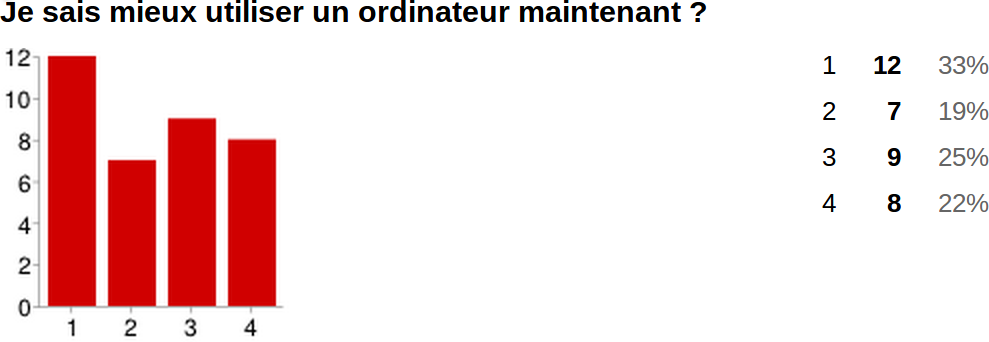
\includegraphics[width=.7\textwidth]{content/8-validation/images/apres}
    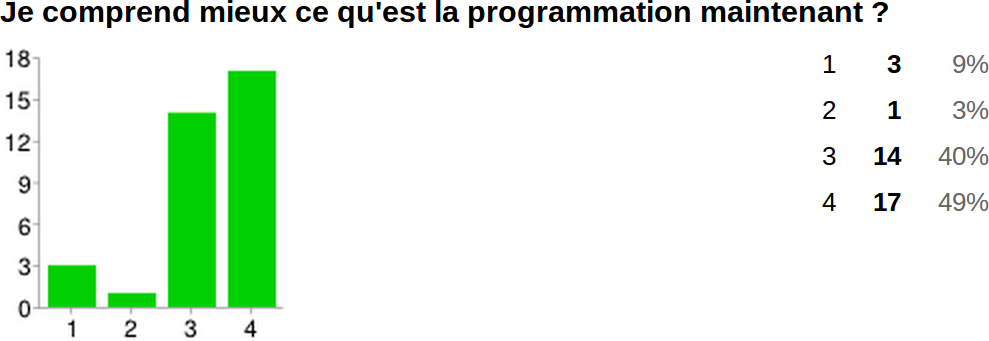
\includegraphics[width=.7\textwidth]{content/8-validation/images/apres-programmation}
    \caption{Auto-estimation du niveau en informatique et en programmation des participants après l'activité}
    \label{fig:niveau-apres}
  \end{center}
\end{figure}

\paragraph{Appréciation des missions}
\label{appreciation}
En plus de l'évaluation de leur niveau de compétences en informatique et en programmation, les participants ont également évalué séparément chaque mission. Les graphiques représentant cette évaluation sont sur la figure \ref{fig:evaluation-mission}. On voit que les missions qui ont été le moins appréciées sont la troisième, "soyons courtois", et la quatrième, "chien et chat".
Sur base des commentaires et de l'appréciation des auteurs, la notation de la quatrième mission peut s'expliquer par la frustration des utilisateurs de ne pas avoir eu le temps de la finir.
Pour la troisième mission, les retours indiquent que les élèves ont trouvé cette mission trop simple. Cette mission pourrait être reconstruite ultérieurement en intégrant, par exemple, le déplacement du personnage.\\


\begin{figure}[ht]
  \begin{center}
    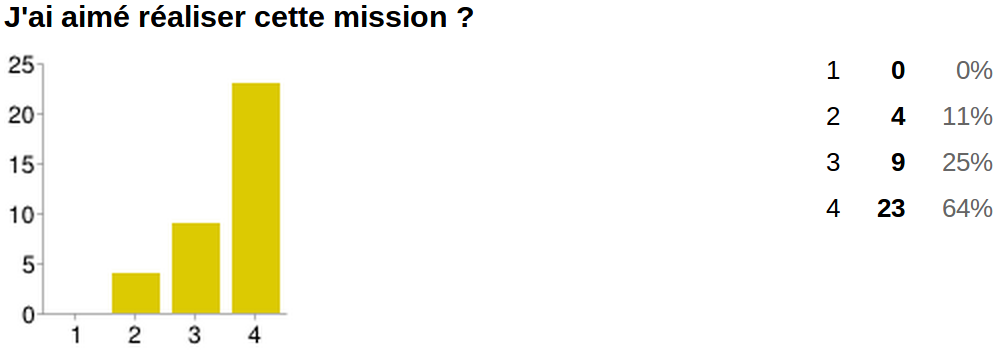
\includegraphics[width=.7\textwidth]{content/8-validation/images/voiture}
    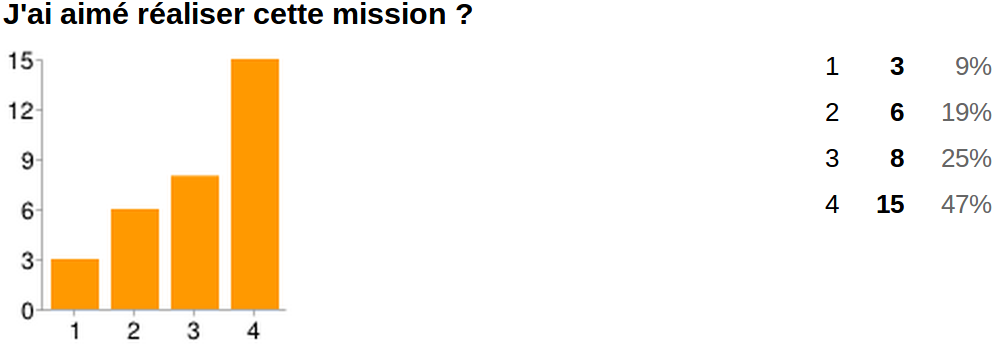
\includegraphics[width=.7\textwidth]{content/8-validation/images/helico}
    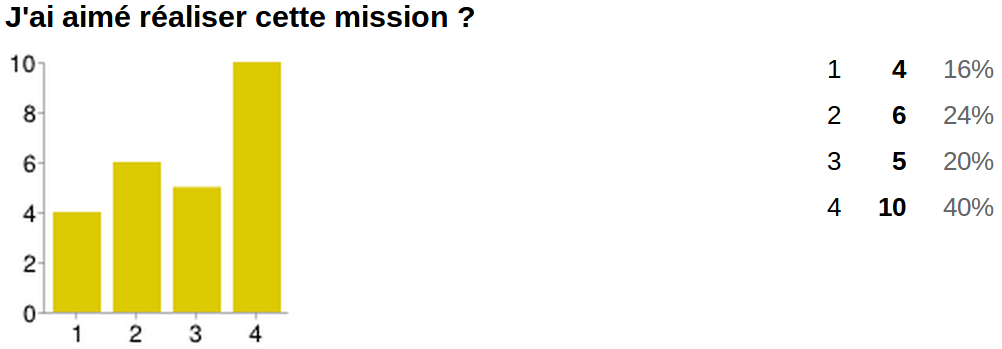
\includegraphics[width=.7\textwidth]{content/8-validation/images/courtois}
    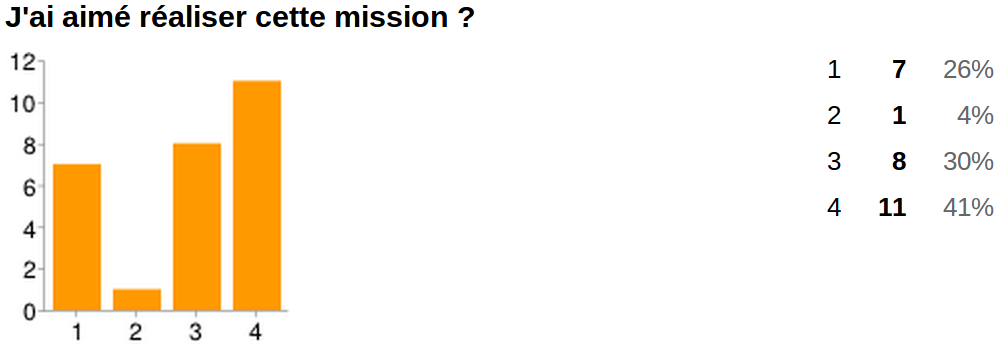
\includegraphics[width=.7\textwidth]{content/8-validation/images/chien}
    \caption{Évaluation des missions par les enfants: En voiture \ref{mission-voiture}, hélicoptère \ref{mission-helicoptere}, soyons courtois \ref{mission-courtois}, tu ne m'attraperas jamais \ref{chien-chat}}
    \label{fig:evaluation-mission}
  \end{center}
\end{figure}

\paragraph{Appréciation des professeurs}
En ce qui concerne les retours des professeurs, voir annexe \ref{result-prof}, ils étaient tous, sans exception, très positifs. Les professeurs d'humanité ont montré beaucoup d'intérêts pour l'utilisation de l'application dans leurs cours. Malgré l'insistance des auteurs, les professeurs n'ont pas donné de critique.

\paragraph{Analyse des missions}
Pour les utilisateurs, la première mission a été la plus laborieuse. Cependant, cette mission a le plus haut taux d'appréciation des enfants. Est-ce du à la facilité de compréhension de cette mission? Est-ce le graphisme? Ou encore son côté concret? Les formulaires n'apportent pas assez d'éléments de réponse.\\

La seconde mission, celle de l'"hélicoptère", a été appréciée, mais, comme cité plus haut \ref{analyse-scienceinfuse}, elle pourrait être séparée en deux missions. En effet, beaucoup d'étudiants ont eu besoin de l'aide des auteurs pour cumuler les deux concepts abordés en une fois.\\

La troisième mission, "soyons courtois", est la moins appréciée. D'après les retours des élèves, elle semble être trop facile. Comme suggéré plus haut \ref{appreciation}, une piste serait de rajouter l'implémentation des mouvements à cette mission.\\

La quatrième mission, "chien et chat", a passionné les élèves mais ils ont été frustrés par le manque de temps. Personne n'a réussi à la finir. Il faudrait peut-être envisager de guider davantage les étudiants dans cette mission. Par exemple, tous les blocs y étaient accessibles, ceci afin que les étudiants puissent découvrir ce qui est possible de faire avec Snap!. L'analyse des questionnaires montre que les étudiants se perdent dans la masse de blocs disponibles.
Une autre possibilité serai d'augmenter le temps imparti à l'expérience tout en tenant compte de la capacité de concentration des enfants. Une durée qui semble intéressante serait deux plages de cinquante minutes.

\paragraph{Tranche d'âge}
\label{trancheage}
Un des objectifs de ce travail est que les enfants utilisent cette application de manière quasi-autonome. Dans ce sens, durant les expériences, les auteurs ont constaté que les enfants de début d'humanité sont plus aptes à travailler de cette manière que les élèves de primaire: moins d'appel à l'aide, plus de persévérance, meilleur prise en charge individuelle, etc.
En conséquence, l'application pour des élèves du fondamental, nécessite soit une plus grande maîtrise de la matière soit plus d'encadrants.

% Les grands vont plus vite

% mission voiture cool pour la structuration
% débouché sur du concret

% différence d'age
% appréciation des missions



%chiffre et analyse de notre formulaire prof et student.



%==========================
%       PART 3
%==========================
\chapter{Conclusions}
Ce chapitre conclut ce mémoire en reprenant les objectifs établis au chapitre \ref{intro-objectifs}. Ces objectifs s'articulaient en trois volets majeurs: plateforme d'apprentissage, contenu et langue et il se finit par un bilan final de ce mémoire.
\section{Plateforme d'apprentissage}
L'objectif était de fournir une plateforme qui permet d'enseigner la programmation aux jeunes de 10 à 14 ans. Cette plateforme doit être disponible partout et être facile d'utilisation. Elle doit également pouvoir stocker des informations pour qu'elles soient disponibles lors de prochaines utilisations.\\

Cet objectif se décompose en plusieurs parties:
\begin{description}
  \item[La portabilité] La plateforme \gls{rsnap} se présente sous la forme d'un site web \cite{rsnap} pour pouvoir y accéder grâce à n'importe quel ordinateur, tablette, etc. Elle est développée en \gls{rails} et JavaScript qui sont des technologies ayant fait leurs preuves, ceci assure une meilleure périnité à la plateforme. Cependant, pour pouvoir bénéficier de toutes les fonctionnalités utilisées par \gls{snap}, il est nécessaire d'avoir un navigateur récent.

  \item[Disponibilité] L'application étant un site web, une connexion à internet est donc nécessaire pour pouvoir avoir accès à la plateforme. Hormis cette contrainte, la plateforme est disponible en tout temps et tout endroit.

  \item[Gestion de classe] L'application fournit déjà la possibilité d'avoir des rôles différents pour les élèves et les professeurs. Ceci permet notamment aux professeurs de gérer la progression des élèves. Cette fonctionnalité est encore un petit peu primitive pour être pleinement utilisable. Elle souffre d'un problème de cloisonnement pour le \gls{role} des professeurs, mais est déjà utilisable pour les élèves.

  \item[L'âge des utilisateurs] Les expériences, voir section \ref{experience}, ont permis de montrer que la plateforme est adaptée à la tranche d'âge visée par ce travail. En effet, les élèves n'avaient aucun mal à passer d'une \gls{mission} à l'autre, sauver leurs projets, les reprendre, etc. Ceci est le fruit des adaptations réalisées grâce aux expériences.
\end{description}

\section{Contenu}
Le contenu comprend toutes les ressources pédagogiques de la plateforme \gls{rsnap}, c'est-à-dire les différentes \glspl{mission} de \gls{rsnap}, mais également les outils pour en créer de nouvelles.

Dans le contenu il est important de différencier les \glspl{mission} existantes des moyens mis en place pour créer ultérieurement du contenu supplémentaire. C'est avec cette subdivision que cette section va aborder le contenu de \gls{rsnap}.

\subsection{Missions existantes}
Cette partie va détailler les concepts enseignés et leur mise en pratique dans les \glspl{mission} déjà proposées.
\begin{description}
  \item[Concepts] Les \glspl{mission} déjà présentes dans \gls{rsnap} introduisent les concepts de base de la programmation tel que les boucles, les conditions et l'enchainement d'instructions. Certains concepts sont moins faciles à maitriser par les enfants. Dans les \glspl{mission} actuelles, il serait avantageux de mieux séparer certains concepts. Par exemple, la \gls{mission} de l'hélicoptère, voir section \ref{mission-helicoptere}, introduit les boucles et les conditions, il serait plus judicieux d'en faire deux \glspl{mission} différentes. Malgré cela tous les enfants ont réussi à réaliser ces \glspl{mission} durant les expériences ce qui montre qu'elles sont déjà bien abouti.

  \item[Mise en pratique] La forme des \glspl{mission} a fortement intéressé les élèves. Des personnages concrets et des retours directs sur leurs actions se sont avérés importants. Les élèves appréciaient, par exemple, que la voiture explose si elle sortait de la route. Ces détails permettent de garder l'enfant attentif et concentré sur les \glspl{mission}.
\end{description}

\subsection{Création de missions}
Cette partie aborde les outils mis en place pour aider à la création de \glspl{mission} supplémentaires.

\begin{description}
  \item[Création de contenu] Pour permettre aux professeurs d'avoir du contenu adapté à leurs besoins, \gls{rsnap} permet de créer leurs propres \glspl{mission}. C'est dans cette optique que des modifications on été opérées sur \gls{snap}, voir section \ref{solution SNAP}. La création de \glspl{mission} par les professeurs a été pensée pour que ces derniers n'aient pas besoin de connaissance spécifique en programmation. En effet, ils créent leurs nouvelles \glspl{mission} directement dans l'interface de \gls{snap}.

  \item[Communauté] La création de \glspl{mission} dans \gls{rsnap} se veut communautaire. En effet comme expliqué dans la section \ref{communaute}, toutes \glspl{mission} crées sont disponibles pour tous les professeurs.
\end{description}

\section{Langue}

Un des points importants de ce travail est qu'il doit être en français pour pouvoir être proposé au plus grand nombre possible d'enfants francophone.

\begin{description}
  \item[Traduction] L'application \gls{rsnap} a été créée et pensée en français. Il est envisageable de traduire cette plateforme. En effet comme elle respecte bien les principes de \gls{rails}, elle est facile à traduire. Les seules parties qui ne pourraient être traduite de manière semi-automatique sont les descriptions des \glspl{mission}. De plus, \gls{rsnap} intègre l'interface de programmation \gls{snap} pour laquelle une traduction partielle existait déjà. Une partie de ce travail a été de compléter cette traduction. Ce travail a d'ailleurs fait l'objet d'une soumission à la communauté de \gls{snap} qui l'a accueillie avec beaucoup d'intérêt.

  \item[Culture] Il est important de souligner que la traduction d'une application dans une langue est plus complexe que la traduction de chaque mot. Une traduction, c'est aussi adapter le contenu à la culture du public cible. La création du contenu de \gls{rsnap} s'est essentiellement inspirée de travaux anglophones, il était donc important de vérifier cette vision sur un public francophone. Les expériences nous montrent que cette adaptation a été réussie pour le contenu proposé.

\end{description}

\section{Bilan final}
Cette section évalue les objectifs de manière plus global, met en lumière les apports de ce travail à l'état de l'art et se finit par une vision du futur de cette application.

\begin{description}
  \item[Objectifs] Dans l'ensemble, les objectifs fixés au début de ce travail ont été atteints, bien que ce genre de travail n'ait jamais de fin. Le résultat est une application qui est déjà utilisable et qui a été appréciée lors des expériences.

  \item[Apport] En plus de proposer une plateforme d'apprentissage de la programmation pour les jeunes francophones, un des apports principaux de ce travail est de montrer que tous les outils nécessaires à sa création sont déjà disponibles individuellement. En effet, la plupart de ces outils sont le fruit d'un besoin de la société de comprendre et maîtriser les technologies qui nous entourent. Ce travail prouve que ces outils peuvent être rassemblés en une plateforme cohérente. Ce pas supplémentaire va dans le même sens que le rapport européen \cite{rapport-europeen} évoqué en introduction.

  \item[Future de Rsnap] Comme dit précédemment, \gls{rsnap} est une plateforme aboutie bien qu'il reste encore beaucoup d'améliorations possibles qui sont abordées dans le chapitre \ref{futur}. Deux futures probables s'ouvrent pour cette application. Soit, elle est reprise par une organisation pour fournir du contenu et du support pour les utilisateurs. Soit, une communauté se crée autour de \gls{rsnap} grâce aux besoins que comble cette application.

\end{description}

\chapter{Future améliorations}
Ce chapitre va aborder les améliorations possibles pour Rsnap. Ces dernières sont soit issues d'objectifs qui n'ont pas été rencontrés par l'implémentation actuelle soit de l'analyse de l'expérience. %TODO pour moi la suite ne sert à rien : Les améliorations suivantes sont à retenir et sont discutées plus dans ce chapitre: test de la réussite de la mission, aide à la gestion de la classe, retravaille et ajout de mission, blocs d'aide a la correction automatique des programmes.

\section{Tester la réussite des missions}
Actuellement, certains tests sont réalisés pour que l'étudiant connaisse la réussite de la mission. Toutes fois, aucun signal n'est envoyé vers les serveurs pour transmettre celle-ci. Une mission est considérée comme réussie dès que l'étudiant ouvre la mission. En effet, comme aucun mécanisme n'est présent pour valider une mission, la mission suivante se débloque dès le premier enregistrement de la précédente.

\paragraph{Modifications à apporter}
Un signal envoyé au serveur serait possible par le simple envoi d'une requête à ce dernier. La difficulté réside dans la création d'un vrai bloc disponible dans l'interface des professeurs qui servirait à notifier le serveur de la réussite de la mission.

\section{Aide à la gestion des groupes}
Un des buts de ce travail est son utilisation dans l'enseignement. Pour ce faire, un système de gestion des élèves par classe a été pensé. Malheureusement, le temps a manqué pour avoir une gestion de groupes finie. 

\paragraph{Modifications à apporter}
Le principe pensé pour la gestion de classe est que chaque professeur puisse voir l'avancement de ses élèves. En plus de l'assignation des étudiants et professeurs à une ou plusieurs classes, il faut aussi que les droits des professeurs ne s'appliquent que pour ses propres étudiants. 

Concrètement, il faut rajouter dans le modèle une classe qui représente un cours. Celle-ci serait constituée de la description de ce cours ainsi que d'un professeur et de plusieurs élèves. Il faut bien sûr aussi modifier les autorités qui gèrent les droits pour tenir compte de ces différentes assignations.

\section{Amélioration et ajout de missions}
Comme mis en lumière dans la partie \ref{analyse-exp}, les expériences ont montré que certaines missions gagneraient à être retravaillées.

\paragraph{Hélocoptère}
La mission de l'hélicoptère introduit deux concepts fort abstraits : les boucles et les conditions. Elle serait beaucoup plus facilement compréhensible par les enfants si elle était découpée en deux parties un pour chaque concept.

\paragraph{Soyons courtois}
La mission soyons courtois n'est pas encore assez attractive pour les enfants. Il était suggéré dans L'analyse \ref{appreciation} de rajouter la programmation des mouvements de leur personnage. En effet, actuellement les autres personnages bougent seuls. On pourrait demander au jeune de programmer ce qui est nécessaire pour que son personnage se déplace grâce au clavier. %TODO c'est déjà fait je comprends pas ce que tu as voulu dire

\paragraph{Chien et chat}
La mission chien et chat n'est pas assez dirigé. Une mission d'introduction supplémentaire serait probablement bénéfique. Un autre problème dans cette mission est le nombre de blocs laissés à disposition des élèves. Le choix avait été fait de leur laisser un accès à tous les blocs pour qu'ils voient la pleine puissance de Snap!. Ce choix s'est révélé inapproprié.

\paragraph{Ajout de missions}
En plus des missions proposées, il est important que d'autres missions soient créées pour avoir un cours consistant. Ces nouvelles missions permettraient d'apporter de nouveaux concepts, mais surtout permettraient aux enfants de pratiquer les concepts déjà appris pour mieux les intégrer.

\section{blocs d'introspection des programmes}
Une idée d'amélioration serait une série de blocs pour avoir des informations sur le programme. Il est déjà possible grâce événements de savoir jusqu'où l'étudiant est arrivé et donc lui attribuer des points en fonction de cela. Pour aller plus loin, il serait intéressant d'avoir un compteur de bloc pour les scripts. En effet, un programme fait avec 20 blocs quand la solution optimale en compte 3 ne mérite probablement pas beaucoup de point.
De manière générale, il serait intéressant d'avoir de vrais blocs disponibles pour les professeurs pour faciliter la création de correction et cotation automatique.

Cette amélioration pourrait être couplée avec le test de réussite. Cette solution enverrait dans la requête au serveur une note et des informations sur l'avancée du programme grâce aux blocs d'introspection.

\section{Charte graphique}
Pour que ce logiciel soit utilisé, il faut porter attention au ressenti des utilisateurs. Un point important est donc d'avoir une charte graphique unifiée et cohérente en fonction du public visé.

\paragraph{Bootstrap et Snap!}
Actuellement, d'une part toute la partie Rails utilise Bootstrap de manière brute, d'autre part l'interface de Snap! n'a été modifié que de manière fonctionnelle. Il serait peut-être judicieux d'adapter un peu la feuille de style de Bootstrap et l'implémentation de Snap! pour avoir un thème graphique unifié et fournir un environnement plus enfantin.

\paragraph{Missions}
Les ressources graphiques utilisées dans les missions proviennent toutes de sources différentes. Avoir un artiste qui dessinerait les différents objets nécessaires permettrait de créer une meilleure unité entre les missions.


% obliger la réussite des test de la mission avant de pouvoir passer à la suivante
% 
% gestion des classes
% 
% rearanger les missions voir analyse
% 
% plus de split dans les missions
% 
% plus de missions
% 
% block de correction automatique des missions
% 
% charte graphique plus cohérente a travers le site et snap! et sur les présentation des missions.



% \appendix
% \glsaddall
% \printindex
% \printglossaries

\nocite{*} %TODO remove
\bibliographystyle{alpha}
\bibliography{biblio}

%\printnomenclature
%\cleardoublepage


\end{document}
